\documentclass[11pt]{article}
\usepackage{mathptmx}
\usepackage[T1]{fontenc}
\usepackage[utf8]{inputenc}
\usepackage{utopia}

\usepackage{geometry}
\geometry{verbose}
\usepackage{units}
%\usepackage{babel}
\usepackage{enumitem}
%%math
\usepackage{amsmath}
\usepackage{amsthm}
\usepackage{amssymb}
\usepackage{stmaryrd}
\usepackage{setspace}
%%tables
\usepackage{booktabs, caption}
\usepackage{threeparttable}
\usepackage{multirow}

%% bibliography management
\usepackage[authoryear]{natbib}
\usepackage{appendix}

\doublespacing
\usepackage[unicode=true,
 bookmarks=false,
 breaklinks=false,pdfborder={0 0 1},backref=section,colorlinks=false]
 {hyperref}

\makeatletter
%%%%%%%%%%%%%%%%%%%%%%%%%%%%%% Textclass specific LaTeX commands.
\newlist{casenv}{enumerate}{4}
\setlist[casenv]{leftmargin=*,align=left,widest={iiii}}
\setlist[casenv,1]{label={{\itshape\ \casename} \arabic*.},ref=\arabic*}
\setlist[casenv,2]{label={{\itshape\ \casename} \roman*.},ref=\roman*}
\setlist[casenv,3]{label={{\itshape\ \casename\ \alph*.}},ref=\alph*}
\setlist[casenv,4]{label={{\itshape\ \casename} \arabic*.},ref=\arabic*}

%%%%%%%%%%%%%%%%%%%%%%%%%%%%%% User specified LaTeX commands.


\usepackage{amsfonts}
\usepackage{eurosym}
\usepackage{ulem}
\usepackage{graphicx}
\usepackage{caption}
\usepackage{color}
\usepackage{sectsty}
\usepackage{comment}
\usepackage{footmisc}
\usepackage{caption}
\usepackage{pdflscape}
\usepackage{subfigure}
\usepackage{array}


\normalem


\newtheorem{hyp}{Hypothesis}\newtheorem{subhyp}{Hypothesis}[hyp]
\renewcommand{\thesubhyp}{\thehyp\alph{subhyp}}

\newcommand{\red}[1]{{\color{red} #1}}
\newcommand{\blue}[1]{{\color{blue} #1}}

\newcolumntype{L}[1]{>{\raggedright\let\newline\\arraybackslash\hspace{0pt}}m{#1}}
\newcolumntype{C}[1]{>{\centering\let\newline\\arraybackslash\hspace{0pt}}m{#1}}
\newcolumntype{R}[1]{>{\raggedleft\let\newline\\arraybackslash\hspace{0pt}}m{#1}}

\makeatother

\providecommand{\casename}{Case}

\begin{document}
\title{\Large{}A Cost-benefit Analysis of R\&D and Patents:
\\ Firm-level Evidence from China\footnote{I am grateful to Mark Roberts and Jonathan Eaton for their guidance and support throughout this project. I thank Paul Grieco and Daniel Grodzicki for their comments at the early stage of this project. I thank Fuxin Zhai and Wenping Zheng for sharing me with the Chinese patents data. All remaining errors are mine. }}
\author{Zhiyuan Chen\footnote{Department of Economics, Pennsylvania State University. Email: chenzhiyuan1224@gmail.com.}}
\maketitle
\begin{abstract}
TBD
\end{abstract}
\textbf{Keywords: }dynamic R\&D investment; patenting; productivity; R\&D subsidy

\newpage

\section{Introduction}

Innovation is a key engine of economic growth. Quantifying the costs and benefits of innovation activities is essential to the understanding of firm's incentives to innovate. Considering the innovation as a process of producing knowledge, R\&D is the input while patents are part of the output. This is formally analyzed in the previous econometric models linking innovation outcome to R\&D investment, and allowing the productivity to be affected by the innovation output \citep{crepon1998research,mairesse2005,raymond2015}. In these models, all of the return to R\&D is captured by the innovation output which is usually measured by patents. However, since only part of the invention is patentable, these studies may obtain a biased estimate for the returns to either R\&D or patents. Moreover, only including R\&D investment in the productivity process gives no room for analyzing the structure of R\&D benefits.

Instead of viewing patents as the only innovation output, this study admits patents as a part of innovation outcome and allows for non-patent inventions to affect the firm's future productivity. In particular, we treat R\&D as the fundamental source of endogenous productivity growth, but the marginal effect of R\&D investment is affected by patent outcomes. Therefore, our specification is an extension of the productivity process considered in the innovation and productivity literature.\footnote{See \cite{hall2010handbook} and references therein for the productivity specifications used in estimating returns to R\&D.} This seemingly small change has ramifications in understanding the structure of returns to R\&D investment. 

Building on the knowledge capital investment model by \cite{hall1989research} and \cite{klette1996r}, the endogenous productivity approach embeds R\&D investment into a stochastic productivity process \citep{Awetal.2011, Doraszelski2013, Peters2017rand}. In particular, the evolution of productivity is modeled as a controlled Markov process: the current R\&D investment increases the average future productivity. Because the current productivity reflects the impact of all distant past R\&D efforts, this approach avoids the problem of calculating the firm-level knowledge stock. With exogenous productivity shocks representing the uncertainty facing innovation, this framework allows for different productivity gains even for firms with identical historical path of R\&D expenditures. Recently, \cite{Peters2017rand} (PRVF hereafter) explicitly analyze different kinds of uncertainty to the innovation process and assume that only the realized innovation affects future productivity. Note a large part of the innovation output is the accumulation of tacit knowledge that are difficult to measure. If this is the case, the productivity shocks in the productivity process will contain the information on R\&D investment that is positively correlated with innovation output. This endogeneity issue can lead to a bias to estimating returns to R\&D investment. 

In this paper, we relax the assumption in PRVF and consider a more realistic setting where both the R\&D investment and innovation output affect the productivity evolution. We follow the main setup of the PRVF model, but have introduced two changes: (1) instead of focusing on directly measured innovation outcome,\footnote{PRVF use the Mannheim Innovation Panel survey which contains the information on the introduction of a new product or a new production process by each firm.} we use patent counts as an important indicator for innovation outcomes; (2) we let productivity be dependent on R\&D even after conditioning on patents. In our framework, R\&D is the fundamental source of productivity change, while the magnitude of its impact is determined by the realization of innovation outcomes. In PRVF, they estimate two primitives regarding the innovation process. The first is the probability of realizing innovation outcome conditional on the state of R\&D investment, and the second is distribution of future productivity conditional on the realized innovation outcome. In our case, we replace the innovation outcome with the firm's patent applications and estimate a similar probability distribution as PRVF.  Moreover, we estimate the distribution of future productivity conditional on both R\&D and patents.

Because the productivity gains depend both on R\&D and realized patent applications, our framework also provides a decomposition of returns to R\&D investment into components related to patents and non-patents, respectively. This leads to an estimator of the private value of patents measured by the increase in the firm value caused by patents. Different from \citet{pakes1986} in which the value of holding a patent is determined by solving an optimal stopping problem, this study measures the expected value of a patent while treating patent applications as a random outcome of R\&D investment. This approach can be applied to any data sets with information on R\&D, patents, and production activities.

We estimate the model using a sample of Chinese high-tech manufacturing firms. Our main findings from the structural estimates are as follows. First, on average R\&D investment causes around 0.45\% increase (or around 0.24 million USD) in the firm value. This value is much lower than that obtained by PRVF, who find that R\&D investment increases firm value by 6.70 percent and 4.41 million Euros for the median high-tech firm in a sample of German firms. This shows that Chinese firms obtain smaller returns to R\&D than German firms. Second, a decomposition of the return to R\&D shows that non-patent innovation accounts for a majority (around 77\%) of the total return to R\&D. Third, the average expected value of an invention (a utility model) patent is around .39 (.34) million USD when measured by the increase in firm value. Lastly, the average start-up cost of R\&D is over ten times larger than the average maintenance cost. This reflects that starting a new innovation project requires a larger amount of investment than maintaining an ongoing research project. Moreover, R\&D costs vary substantially across different industries, with electronics sector being the highest.

Using the estimated model, we perform a series of counterfactual exercises to evaluate the effectiveness of different types of R\&D subsidy policies that reduce R\&D costs. In particular, we compare the effect of per unit lump-sum subsidy and proportional subsidy.\footnote{The lump-sum subsidy is a fixed amount of government transfer that reduces R\&D costs paid by the firm, while the proportional subsidy is a reduction in R\&D costs at a fixed proportion. If the amount of R\&D costs is $c$, the lump-sum subsidy reduces R\&D costs to $c-s_l$, and the proportional subsidy changes the R\&D costs to be $(1-s_p)c$.} Some interesting results are found. First, for both types of the subsidy programs, a reduction in maintenance costs causes a greater increase in the firm value. But subsidizing start-up (maintenance) costs promotes innovation participation more under lump-sum (proportional) subsidy. Second, lump-sum subsidy is more efficient than proportional subsidy. In the experiment of 20\% decrease in maintenance costs for R\&D, the average efficiency of lump-sum subsidy is around 12 times greater than the proportional subsidy in increasing the firm value, and is about twice greater in promoting the firm's innovation participation. The difference is more striking when we consider the subsidy for start-up costs of R\&D. 

This study is closely related to the literature on quantifying returns to R\&D. The knowledge capital model of \citet{griliches1979issues} has been a corner stone of this literature. In this framework, the investment in innovation by the firm creates knowledge stock, which is similar to physical capital in the way that they enter into the production function. The most important extension related to this paper is the econometric framework proposed by \citet*{crepon1998research} (CDM hereafter) which estimates a reduced-form model incorporates R\&D, patents, and productivity. Recently, \citet*{raymond2015} have extended this  framework to a dynamic setting. However, the knowledge-stock approach faces the problem of estimating the firm's knowledge stock. It also rules out the high degree of intrinsic  uncertainty facing innovation investment. 

We contribute to the existing literature in several aspects. First, it enriches the literature on quantifying returns to R\&D by providing a decomposition of the benefits of R\&D into patenting and non-patenting channels. The empirical finding suggests that non-patenting R\&D investment plays a major role in returns to R\&D. Second, we provide a new method of quantifying the private value of patents. Third, the empirical implementation in this paper provides a first structural analysis on the costs-benefits structure of R\&D and patents in China, thus contributing to the literature on understanding the innovation activities in China.\footnote{See, for example, \cite{Hu2009}, \cite{Hu2017}, and \cite{chen2017}.} The estimation results show that non-patents innovation accounts for most of returns to R\&D. Moreover, the relative small benefits of R\&D activities and relatively high start-up R\&D costs jointly help explain low participation in investing R\&D. 

The rest of this paper is organized as follows. In Section 2, we outline the R\&D model and the method of decomposing R\&D benefits and estimating the patent value. Data are introduced in Section 3. Section 4 provides the empirical results.  Section 5 is the counterfactual analysis on the effectiveness of R\&D subsidies. Section 6 concludes the paper. 

%-------------------------------------
%Section 2: The Empirical Framework
%-------------------------------------

\section{The Empirical Framework}

In this section, we first briefly lay out a standard dynamic model of R\&D investment and patent outcomes. The basic structure of the model is identical to PRVF, the only difference is that we allow that both R\&D and patents play a role in shifting the distribution of future productivity. Then we provide a decomposition of returns to R\&D as well as a quantification of the patent value. 

\subsection{Model}
In PRVF, a firm's R\&D decision changes the probability of realizing product or process innovations, which affect the firm’s future productivity and expected
profits. In their specification, only the innovation outcome (process or product innovation) caused by R\&D activities has an impact on the firm’s future productivity and hence future profits. In contrast, we allow both R\&D and patents enter the productivity evolution equation while the creation of new ideas represented by observed patent applications affects the marginal effect of R\&D on future productivity. 

The model comprises of four parts. The first part is the firm’s patents production function that links the distribution of patents to R\&D investment by the firm. The second component is the cost function of investment in R\&D, which is influenced by the previous experience in R\&D. The third component of the model links a firm’s patent activities with the process of productivity evolution, in which patents and R\&D alter the probability distribution of the firm’s future productivity. The last component of the model expresses the profits as a function of current R\&D activities and future productivity. In equilibrium, each firm chooses the optimal level of investment in R\&D to maximize its expected profits.\footnote{As I show in the appendix, this framework can easily be extended to accommodate the adjustment of R\&D investment at the intensive margin.}

\textit{R\&D-patents linkage.} A firm can affect the output of patents and further affect the evolution of
productivity and profits through participating in R\&D activities. We define two binary variables $n_{it}$ and $b_{it}$ , where $n_{it}$, $b_{it}$ $\in\{0,1\}$, to capture patents for inventions and utility models, respectively. $n_{it}=1$ ($b_{it}=1$) if firm $i$ produces invention (utility model) patents in year $t$. The linkage
between R\&D and patents is modeled as a cumulative joint distribution of invention patents and utility model patents conditional on the past decision on R\&D, $P(n_{it+1}, b_{it+1}|rd_{it})$.

By formulating the R\&D-patent linkage as a conditional joint cumulative distribution function, we implicitly take the correlation between invention patents and utility patents into consideration. This can be caused by the idea diffusion within the firm. We also expect that firms engaging in R\&D activities are more likely to produce invention or utility patents. Lastly, we do not model the possibility that different firms have different inclination to protect their ideas by creating patents. However, we try to alleviate the concern that some firms may not want to protect their innovation via patenting by focusing on high-tech industries, with the hope that high-tech firms are more willing to file patent applications when they have new ideas. In addition, our sample period starts from 2002, before which China has implemented several amendments to patents law aimed to strength the protection of intellectual property rights \citep{Hu2009}. As a result, our measure is an average of the industry-specific propensity of submitting patent applications.

\textit{Firm's revenue and profits.} The demand is CES with an elasticity of substitution being $\sigma$. The log of firm's short-run revenue from selling products is given by:
\begin{equation} \label{log-rev}
    r_{it} =(\sigma-1)(\beta_k k_{it}+\beta_aa_{it}+\phi_{it}) +\mu_0+\mu_t
\end{equation}
where $k_{it}$ is the log of the firm's capital stock, and $a_{it}$ is the firm age.\footnote{See Appendix B for the detailed derivation.} $\mu_0$ is a constant term. $\mu_t$ is a year-specific variable common to all firms, which contains information on factor prices. $k_{it}$ is treated as a fixed factor in the short-run. $\phi_{it}$ represents the revenue productivity, which includes firm's production efficiency as well as the idiosyncratic demand shifter. The firm's short-run profits is:
\begin{equation}
    \pi_{it} = \frac{1}{\sigma}\exp(r_{it})
\end{equation}

\textit{Productivity evolution.} we modify the process of productivity evolution in PRVF and assume that both past R\&D activity and current patent counts affect future productivity. Specifically, the distribution of future productivity is affected by a firm’s past productivity ($\phi_{it}$) and R\&D activities ($rd_{it}$) and logs of the current realization of invention patents ($n_{it+1}$) and utility model patents ($b_{it+1}$). As an extension to existing literature, we allow both R\&D activity and patent activities enter into the productivity evolution equation. In my specification, the effect of R\&D investment on future productivity depends on the patents.Specifically, the evolution equation of firm productivity is as
following:

\begin{equation}
    \phi_{it+1} = h(\phi_{it}, rd_{it}, rd_{it}\times n_{it+1}, rd_{it}\times b_{it+1}) + \varepsilon_{it+1},
\end{equation}
where $h(\phi_{it}, rd_{it}, rd_{it}\times n_{it+1}, rd_{it}\times b_{it+1})$ is the conditional mean of future productivity and $\varepsilon_{it+1}$ is an i.i.d stochastic shock normally distributed with zero mean and variance $\sigma_{\epsilon}^2$. This
formulation assumes that (1) a firm’s productivity is persistent over time, implying that future productivity will be correlated with its current productivity; (2) R\&D and patent counts jointly shift the mean of future productivity, with R\&D being the fundamental source of endogenous productivity change; and (3) productivity change is influenced by stochastic shocks $\varepsilon_{it+1}$. More importantly, I allow the impact of R\&D on the future productivity depends on the outcome of patents. To account for the difference between invention patents
and utility model patents in affecting the firm’s future productivity, we allow that $\partial h/\partial n_{it+1}$ and $\partial h/\partial b_{it+1}$ to be different. It is worth noting that the formulation of productivity process is different from that considered in PRVF. In the specification of PRVF, only the innovation outcomes enter into the productivity evolution process. In other words, R\&D investment can only affect the productivity evolution through the measured innovation outcome. In our setting, it is clear that R\&D is the fundamental source of productivity growth, but the magnitude of its impact is determined by the innovation outcome. Therefore, R\&D investment has both direct and indirect effect on the productivity. PRVF end up estimate two primitives via a two-step procedure: (1) $\Pr(innovation| R\&D)$, and (2) $\Pr(productivity|innovation)$. 

\textit{R\&D costs and equilibrium.} Following PRVF, the innovation cost is assumed to be dependent on prior R\&D experience and current capital stock. For firm $i$ in year $t$, its innovation cost $C_{it}$ is given as:
\begin{equation}
    C_{it}\sim \exp(\kappa_m\times rd_{it-1}\times k_{it}+\kappa_{s}\times(1-rd_{it-1})\times k_{it}),
\end{equation}
where $\exp(\cdot)$ represents the exponential distribution. Hence the cost of investing in R\&D follows an exponential distribution with a mean of $\kappa_mk_{it}$ when $rd_{it-1}=1$, and with a mean of $\kappa_sk_{it}$ when $rd_{it-1}=0$. $\kappa_m$ and $\kappa_s$ can be different, implying that the distribution of
maintenance costs differs from start-up costs. $\kappa_sk_{it}$ captures the start-up costs when a firm did not participate in R\&D activities in the previous period but plan to undertake R\&D investment in the current period. In contrast, $\kappa_mk_{it}$ reflects the maintenance costs when a firm was active in R\&D investment in the previous period and continue to invest in R\&D.  $k_{it}$ enters the distribution of R\&D costs because of the scale effect that a firm with larger capital stock are required to hire more researchers and build larger research labs. Throughout the estimation, we treat $k_{it}$ to be exogenous. The state variables are $s_{it} = (\phi_{it} ,rd_{it-1})$. The firm’s decision on R\&D will affect the evolution of $s_{it}$. The firm’s value function $V(s_{it})$ can be calculated as:
\begin{align}
    V(s_{it}) &= \pi(\phi_{it}) + \\
              &\beta \int _0^{\infty}\max_{rd_{it}}\left\{\mathbf{E} V(s_{it+1}|\phi_{it},rd_{it}=1)-C_{it}, \mathbf{E}V(s_{it+1}|\phi_{it}, rd_{it}=0)\right\}dG(C_{it}) \nonumber
\end{align}
where $\beta$ is the discount factor. We define $\gamma_{it}$ as the parameter for the exponential distribution:
\[
\gamma_{it}\equiv \kappa_m\times rd_{it-1}\times k_{it}+\kappa_{s}\times(1-rd_{it-1})\times k_{it},    
\]
then $G(C_{it})=1-\exp(-C_{it}/\gamma_{it})$ for $c\geq0$ and zero otherwise. The expected future value of the firm is an expectation over the future productivity levels and the count of patent applications:
\begin{equation}\label{vf}
    \mathbf{E}V(s_{it+1}|s_{it}) = \sum_{n_{it+1}}\sum_{b_{it+1}}\int_\phi' V(s_{it+1})dF(\phi'|\phi_{it}, n_{it+1}, b_{it+1}, rd_{it}) P(n_{it+1}, b_{it+1}|rd_{it})
\end{equation}

Note that (\ref{vf}) is composed of two parts representing two kinds of uncertainties facing innovation. The first uncertainty comes from the creating of applicable patents (or creating new ideas); the second uncertainty comes from the response of future productivity to the future patenting activities and R\&D decision in the previous year. The firm maximized its firm value, which implies that a firm will choose to invest in R\&D if and only if

\begin{equation}
    \Delta EV(\phi_{it}) \equiv \mathbf{E} V(s_{it+1}|\phi_{it}, rd_{it}=1)-\mathbf{E} V(s_{it+1}|\phi_{it},rd_{it}=0)\geq C_{it}
\end{equation}

In equilibrium, a firm will only invest in R\&D as long as the expected net benefit from R\&D is greater than the costs.

\subsection{R\&D benefits decomposition and patent value}
\textit{R\&D benefits decomposition.} Given the structure of the model, we decompose the benefits of R\&D into components related to patent counts. One novelty of the current paper is the quantification of returns to R\&D through patent and non-patent channels. Following PRVF, the long-run benefits of R\&D are measured as the relative change in the expected firm value caused by R\&D investment:
\begin{equation}
    LB(\phi_{it}) = \frac{\mathbf{E}V(s_{it+1}|\phi_{it}, rd_{it}=1)-\mathbf{E}V(s_{it+1}|\phi_{it}, rd_{it}=0)}{\mathbf{E}V(s_{it+1}|\phi_{it}, rd_{it}=0)}
\end{equation}

Note that conditioning on that a firm is undertaking R\&D investment, its firm value is calculated as a weighted average of different states of realization of patents $(n_{it+1}, b_{it+1})$. In case when the patent count is zero and the firm is active in R\&D investment, that is $(n_{it+1}, b_{it+1}, rd_{it})=(0, 0, 1)$, the non-patent channel through which R\&D benefits are realized can be computed as:
\begin{equation} \label{LB_N}
    LB_N(\phi_{it}) = P(0,0|1)\int_{\phi'}V(s_{it+1})dF(\phi'|\phi_{it}, 0, 0, 1),
\end{equation}
Similarly, the R\&D benefits realized through the patent channel is:
\begin{equation} \label{LB_P}
    LB_P(\phi_{it}) = \sum_{\left\{n',b': n' + b' >0\right\}}P(n',b'|1)\int_{\phi'}V(s_{it+1})dF(\phi'|\phi_{it}, n', b', 1)
\end{equation}

While the benefits of R\&D ($LB$) are interesting by themselves, the decomposition of $LB$ into the patent and non-patent channel provides a deeper view of the internal structure of R\&D benefits. Since $LB_p$ contains information on the firm's patent value that is reflected in the productivity growth, the relative importance of $LB_p$ in total R\&D benefits is closely related to the quality of patent system. When $LB_N$ plays a dominant role in the total benefits of R\&D, we can expect that the value of patent is not so valuable and most of the R\&D benefits are realized through knowledge accumulation through non-patent activities.

\textit{Patent value.} In \cite{pakes1986}, the distribution of returns from holding patents is estimated by solving the patentee’s optimal stopping problem of whether renewing the patent or not. Introducing patent counts into the productivity evolution enables us to analyse the patent value using a new approach. To obtain the value of patents, we need to condition on firm’s R\&D investment since R\&D is the fundamental source of productivity growth. After conditioning on the R\&D investment, we compute the increase in the firm value caused by the change in the patent counts. Following this logic, the long-run value of an invention patent is given by
\begin{align} \label{vp_inv}
    VP_{inv}(\phi_{it}) =& \ln \underbrace{\left[\sum_{b'\in\{0, 1\}}\Pr(b'|n_{it+1}=1)\mathbf{E}V(s_{it+1}|\phi_{it}, 1, b', 1)\right]}_{\text{firm value when an invention occurs: }VP_{inv}^1(\phi_{it})} \\
                         & - \ln \underbrace{\left[\sum_{b'\in\{0, 1\}}\Pr(b'|n_{it+1}=0)\mathbf{E}V(s_{it+1}|\phi_{it}, 0, b', 1)\right]}_{\text{firm value when no invention occurs: }VP_{inv}^0(\phi_{it})}, \nonumber                
\end{align}
where $\Pr(b'|n_{it+1} = n')$ is the probability of the event $b_{it+1} = b'$ conditional on $n_{it+1} = n'$. In a similar way, we can compute the value of a patent of utility model:
\begin{align} \label{vp_uti}
    VP_{uti}(\phi_{it}) = &  \ln \underbrace{\left[\sum_{n'\in\{0, 1\}}Pr(n'|b_{it+1}=1)\mathbf{E}V(s_{it+1}|\phi_{it}, n', 1, 1)\right]}_{\text{firm value when a utility model occurs: }VP_{uti}^1(\phi_{it})} \\
                         &-\ln\underbrace{ \left[\sum_{n'\in\{0, 1\}}Pr(n'|b_{it+1}=0)\mathbf{E}V(s_{it+1}|\phi_{it}, n', 0, 1)\right]}_{\text{firm value when no utility model occurs: } VP_{uti}^0(\phi_{it})}. \nonumber  
\end{align}
Then the expected firm value when a firm invests in R\&D can be decomposed as:
\begin{align}
    \mathbf{E}V(s_{it+1}|\phi_{it}, rd_{it}=1)=& \Pr(n_{it+1}=1)VP_{inv}^1 + (1-\Pr(n_{it+1}=1))VP_{inv}^0 \\
                                              =& \Pr(b_{it+1}=1)VP_{uti}^1+ (1-\Pr(b_{it+1}=1))VP_{uti}^0, \nonumber
\end{align}
where the unconditional probabilities $\Pr(n_{it+1}=1) = P(1, 0|1)+P(1,1|1)$ and $\Pr(b_{it+1}=1) = P(0, 1|1)+P(1,1|1)$. In principle, the patent value is defined for each firm. Even if this firm does not submit any patent applications, the formulae (\ref{vp_inv}) and (\ref{vp_uti}) delivers the shadow value of a potential patent. To make the results comparable with existing literature, one can estimate the value of patent focusing on observations with positive counts of patent. 

In what follows, we employ the empirical framework to analyze a sample of Chinese high-tech manufacturing firms. We first introduce the data source, then we explain the estimation procedures and the estimation results. 

%-----------------------
%Section 3 Data
%-----------------------

\section{Data}
\subsection{Data sources}
\textit{Firm-level production data.}
The first data set contains information on the large and medium sized Chinese manufacturing firms from 2001 to 2007 complied by China's National Bureau of Statistics (CNBS hereafter). This data set is widely used in studies on Chinese firms (See \cite{HsiehKlenow}, \cite{song2011}, and \cite{BRANDT2012339} for example). This data set includes all Chinese State Owned Enterprises (SOEs hereafter) and non-SOEs with annual sales no less than five million \textit{Renminbi} (equivalent to about 700,000 US dollars). These firms accounts for 98\% of the manufacturing exports. This data set contains all the information of the firm's major accounting sheets, which includes more than 100 financial variables. Serving for the purpose of this study, it includes firm sales, number of employees, material input, fixed assets, R\&D expenditures, and other firm characteristics like firm age and its industrial code. In summary, this rich data set provides information on the firm-level production activities. We have obtained a sample of high-tech manufacturing firms from this dataset. 

\textit{Patent data.} The second database is on patent statistics collected by the State Intellectual Property Office (henceforth SIPO) of China. It contains
all the patents that are applied by Chinese firms and granted in mainland China. For each patent the database provides information on its type (invention, utility model, and design), owner, application time, certification time, agent of application, abstract, location, and expiration time during 1985 and 2012. But it should be noted that there is no information on citations for patents in the database,
which makes it difficult to measure the patent quality directly. According to China's Patent Law, the utility model refers to a new technical solution suitable for practical use proposed for the shape, construction or combination of the products.\footnote{According to WIPO, utility models are sometimes referred to as ``short-term patents'', ``utility innovations'' or ``innovation patents''......In general, utility models are considered particularly suited for protecting inventions that make small improvements to, and adaptions of, existing products or that have a short commercial life.}  Generally, an invention patent is also related to a new technical solution proposed for the product, method or its improvement. But the patenting process for invention patent consists of a``substantive review'' which specifically emphasizes on the novelty and originality of the breakthrough in technical upgrading. Obviously, lower creativity standards are enforced for utility model patents.As for design patents, they represent more rudimentary type of innovation and are considered to be of lower quality than invention patents and utility model patents.\footnote{ According to Article 22 of the Patent Law of the P.R.C.: any invention
or utility model for which patent right may be granted must possess
novelty, inventiveness and practical applicability. In comparison,
the requirement for the approving of design patents is in Article
24 of the Patent Law of the P.R.C as \textquotedblleft \dots \dots must
not be identical with or similar to any design which, before the date
of filing, has been publicly disclosed in publications in the country
or abroad or has been publicly used in the country, and must not collide
with any legal prior rights obtained by any other person.\textquotedblright{}}
 Therefore we anticipate that design patents is less related to firm's productivity. Considering this, we focus on invention patents and utility patents in the empirical investigation. 

\textit{Final combined database.}
We merge the aforementioned two data sets using the
firm name. Table \ref{T1} shows aggregate information on the number of patents for the combined database. The aggregate number of invention patents and utility patents show a strong increasing trend over the sample period. One important concern on using the combined data set is the
efficiency of matching between these two data sets. To evaluate the
matching efficiency, in the last row of Table \ref{T1}, we show the percentage of the total number of invention patents in the merged data set to
the figure published in the China Statistical Yearbook on Science
and Technology. We find that this ratio varies across years, with
55.57\% in 2007 and 96.35\% in 2003. Overall, the merged data set captures most of the information in the patents data. Because the patent counts published in China Statistical Yearbook also reflect many firms that are either small firms or non-manufacturing firms, we find that our results are reasonable. 

\begin{table}[h]
    \caption{Patent counts in the merged database and matching efficiency}
    \label{T1}
    \begin{centering}
    \begin{tabular}{clllllll}
    \toprule
    year & 2001 & 2002 & 2003 & 2004 & 2005 & 2006 & 2007\\
    \hline
    invention & 1982 & 4462 & 5333 & 7993 & 10100 & 17033 & 19750 \\
    utility model & 4202 & 5649 & 7496 & 7798 & 10720 & 15324 & 18212\\
    \hline
    matching  & 57.10\% & 81.26\% & 96.35\% & 87.20\% & 57.58\% & 67.33\% & 55.67\% \\
    \bottomrule
    \end{tabular}
    \par\end{centering}
    {\small{}Note: matching efficiency refers the ratio of number of invention patents in the merged data set to the published figures in China Statistical
    Yearbook on Science and Technology 2001-2007.}{\small \par}
\end{table}

\subsection{Descriptive statistics}
China's high-tech industries mainly covers four 2-digit industries: pharmaceutical manufacturing, special equipment, electric machinery, and electronics. In Table \ref{T2} we report the summary statistics for the R\&D and patenting activities in the final dataset. The average R\&D expenditure for high-tech manufacturing firms is 218.095 thousand yuan (equivalent to around 31,584 US dollars). The R\&D intensity measured by total R\&D expenditures over total sales is lower than that reported for developed countries. Lastly, compared to the R\&D participation, we observe that the probability of generating a patent is relatively low. Even for high-tech firms, the pooled probability of generating an invention patent application is only 5.6\%.  

\begin{table}[h]
    \caption{Summary statistics for high-tech and non-high-tech industries}
    \label{T2}
    \begin{centering}
    \begin{tabular}{lllll}
    \toprule
     & \multicolumn{2}{c}{High-tech} & \multicolumn{2}{c}{Non-high-tech} \\ \cmidrule{2-5}
    Variable & Mean & Std. Dev. & Mean & Std. Dev.\\
    \hline
    R\&D expenditures & 218.095 & 963.152 & 34.886 & 326.677\\
    R\&D/employees & 1.794 & 8.327 & 0.282 & 4.686\\
    R\&D/sales & 0.007 & 0.024 & 0.001 & 0.008\\
    Pr(R\&D>0) &0.289 & 0.454 & 0.106 &0.307 \\
    Inventions & 0.056 & 0.776 & 0.010 & 0.306\\
    Utility models & 0.083 & 1.058 & 0.028 & 0.376\\ \bottomrule
    \end{tabular}
    \par\end{centering}
    {\small{}Note: the unit of R\&D expenditures is 1,000 yuan (around
    150 US dollars).}{\small \par}
\end{table}

In Figure \ref{F1}, we display the number of firms for each 2-digit high-tech industry
by their innovative activities. As shown in Figure \ref{F1}, even
for the high-tech manufacturing firms in China, only a small portion of firms
undertake R\&D investment. The fraction
of firms that file patent applications is even smaller. The difference
between R\&D activities and patent applications implies that distinguishing
the input of innovation and output of innovation is important when
considering the costs and benefits of innovation because R\&D activities with patents may generate a larger impact on the firm's productivity. The sharp decline in the number of firms also suggests that innovative firms face a large degree of uncertainty in generating patents. 

\begin{figure}[h]
    \caption{Number of Firms by Innovation Activities} 
    \label{F1}
    \begin{centering}
    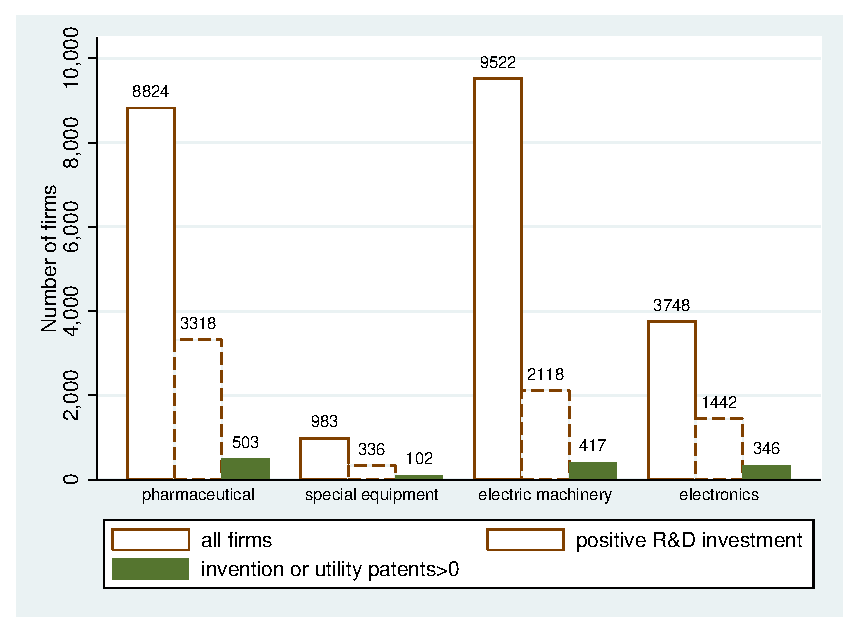
\includegraphics[width=0.7\textwidth]{Figs/FirmsCount.eps}
    \par\end{centering}
    \caption*{\small{}Note: numbers are from the final database}{\small \par}
\end{figure}

\subsection{Quality of R\&D data}
\cite{mairesse2005} provide evidence on the substantial measurement error of using R\&D expenditures to predict the innovation probability for the firm-level data from the French innovation survey. More related, \cite{chen2017wp} document that corporate income tax reductions induce Chinese firms to relabel administrative expenses as expenditures on R\&D. These results suggest that the levels of R\&D may not accurately reflect the firm's actual investment in innovation. In appendix \ref{app_data_features}, we also show that the extensive margin of R\&D and patents captures most of the innovation effects. Therefore we prefer using information on the R\&D choice at the extensive margin as PRVF did. The estimation methodology does not require the researchers to have information on the intensive margin of R\&D investment. Instead, it assumes that the econometrician is ignorant about the true R\&D costs paid each firm, therefore to some extent it is robust to measurement errors in R\&D data at the intensive margin. As long as the extensive-margin status of R\&D is measured correctly, the PRVF method still holds when the distribution of R\&D costs is well assumed. 

In the model, a firm's current state includes its R\&D choice in the previous period.  Firm $i$ is undertaking start-up R\&D if $(rd_{it-1}, rd_{it})=(0, 1)$, and is participating maintenance R\&D if $(rd_{it-1}, rd_{it})=(1, 1)$. The start-up R\&D is not literally the innovation expenses for a new project as we do not have information on the operation of research projects by each firm. In this sense, our definition of different types of R\&D is loose and only reflects the continuity of R\&D investment in a two-period fashion. To prepare the data for estimation, we require that a firm exists at least for two consecutive years to identify the firm's R\&D status in the past and current periods. In Figure \ref{fig:rd_transition}, we show the probabilities for start-up and maintenance R\&D. A universal pattern is that most firms (around 80\%) tend to continue their R\&D investment, but many less firms (around 10\%) perform start-up R\&D. This implies that firms face a large adjustment cost for R\&D investment, which is consistent with the R\&D literature documenting that firms tend to smooth R\&D spending over time because of the long time between conception and commercialization \citep{hall1986patents,lach1989dynamics, hall2010handbook}.

\begin{figure}[h]
    \centering
    \caption{Transition probability for start-up and continuing R\&D}
    \label{fig:rd_transition}
    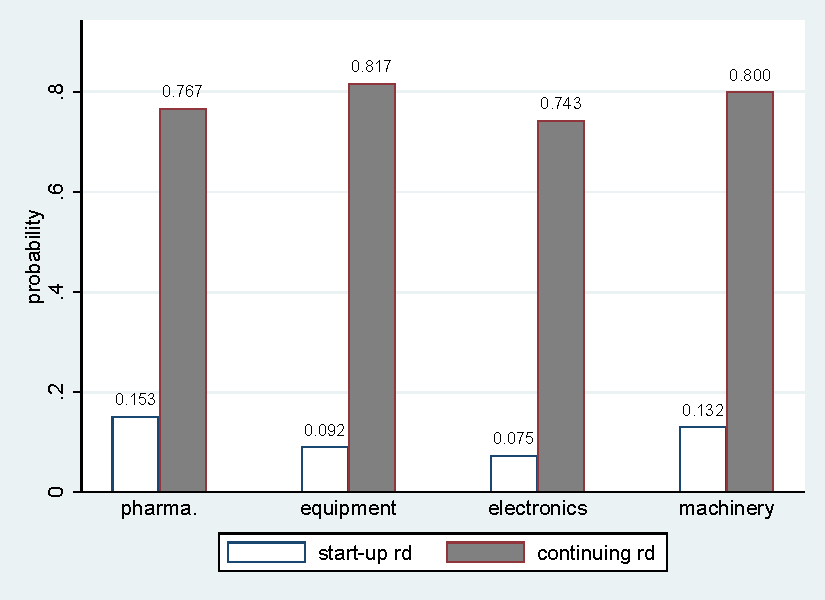
\includegraphics[width=0.7\textwidth]{Figs/rd_prob_transition.pdf}
\end{figure}


\section{Estimation and Results}
The empirical method we use follows PRVF closely with only one exception: we include both R\&D and patents in the productivity evolution. In PRVF, they estimate to primitives regarding the impact of R\&D investment: (1) Pr(innovation|R\&D), and (2) Pr(productivity|innovation). In our case, we still estimate (1), but (2) becomes the distribution of productivity conditional on innovation and R\&D investment. Instead of using a direct measure of innovation outcome, we use patent counts as the indicator for innovation. As for analyzing the estimation results, we provide the decomposition of R\&D benefits and the value of patents in addition to the total R\&D benefits. To simplify the notation, we will omit time and firm subscripts whenever no confusion arises. Without special notice, $Z'$ represents the next-period $Z$, and $z=\ln (Z)$.

\subsection{Productivity estimation}

\textit{Revenue equation.}
We parameterize the productivity evolution process as a cubic function of lagged productivity:

\begin{align} \label{mk}
\phi_{it+1} =& \rho_{0}+\rho_{1}\phi_{it}+\rho_{2}\phi_{it}^{2}+\rho_{3}\phi_{it}^{3} \\
             & +\rho_{4}rd_{it}+\rho_{5}\left(n_{it+1}\times rd_{it} \right)+\rho_{6}\left(b_{it+1}\times rd_{it}\right)+\varepsilon_{it+1}, \nonumber 
\end{align}
where the first line on the right-hand side captures the persistence
in productivity trajectory, the second line describes the impacts of R\&D and
patents on the evolution of productivity. It is clear that past R\&D activity and patent counts jointly affect the future productivity. In particular, we have $\frac{\partial^2 \phi_{it+1}}{\partial rd_{it}\partial n_{it+1}}=\rho_5$ and $\frac{\partial^2 \phi_{it+1}}{\partial rd_{it}\partial b_{it+1}}=\rho_6$. These two second-order partial derivatives clearly state that the impact of R\&D investment (the innovation input) on productivity is affected by patents (the innovation outcome). We expect
that $\rho_{5}$ and $\rho_{6}$ are different from each other because
different types of patents represent different forms of realized innovation. These two
parameters also give us information on the quality of patents and the effectiveness of patenting system. When they are positive, patents help strengthen the productivity effect of R\&D investment. It is also possible that they are positive, implying that submitting patent applications actually weakens the productivity premium caused by R\&D investment.\footnote{This may be because of the leakage of key information on production technologies to the firm's competitors, which ultimately pulls down the demand facing the firm and reduces the revenue productivity.} 
I estimate the productivity using the first-order condition of materials.The demand for materials is dependent on the observed capital stock, age, and unobserved productivity. This gives us an expression for the productivity:
\begin{equation}
\phi_{it-1}=\left(\frac{1}{1-\sigma}\right)\beta_{t-1}+\beta_{k}k_{it-1}+\beta_{a}a_{it-1}-\frac{1}{1-\sigma}m_{it-1}\label{productivity}
\end{equation}
where $\beta_{t}$ represents the the intercept of the CES demand function and the price of variable inputs common to all firms. Combining (\ref{mk}) and (\ref{productivity}), then plugging them into (\ref{log-rev}) yields an empirical equation for
the firm revenue:
\begin{align} \label{nls}
r_{it}=& \left(1-\sigma\right)\beta_{k}k_{it}+\left(1-\sigma\right)\beta_{a}a_{it}  \\
       &-\rho_{1}\left[\beta_{t-1}+\beta_{k}\left(1-\sigma\right)k_{it-1}+\beta_{a}\left(1-\sigma\right)a_{it-1}-m_{it-1}\right] \nonumber \\
 & -\frac{\rho_{2}}{1-\sigma}\left[\beta_{t-1}+\beta_{k}\left(1-\sigma\right)k_{it-1}+\beta_{a}\left(1-\sigma\right)a_{it-1}-m_{it-1}\right]^{2} \nonumber \\
 & -\frac{\rho_{3}}{\left(1-\sigma\right)^{2}}\left[\beta_{t-1}+\beta_{k}\left(1-\sigma\right)k_{it-1}+\beta_{a}\left(1-\sigma\right)a_{it-1}-m_{it-1}\right]^{3} \nonumber \\
 & -\left(1-\sigma\right)\left[\rho_{4}rd_{it-1}+\rho_{5}\left( n_{it}\times rd_{it-1}\right)+\rho_{6}\left( b_{it} \times rd_{it-1}\right)\right]+ \mu_{0}+\mu_{t}+v_{it} \nonumber 
\end{align}
where $v_{it}=u_{it}-\left(1-\sigma\right)\varepsilon_{it}$, with 
$u_{it}$ being the measurement error to the revenue and exogenous to
the firm's decisions on choosing variable inputs or investment in
R\&D. The estimation of (\ref{nls}) relies on the condition that
the composite error $v_{it}$ is uncorrelated with all the explanatory
variables on the right-hand side. $\mu_{0}$ is an intercept which
combines constants from the revenue function and the productivity
process. $\mu_{t}$ and $\beta_{t-1}$ are functions of the common
time-varying variables including the demand intercept and factor prices. The higher-order powers on $\phi_{it-1}$ enables us to distinguish $\beta_{t-1}$ from $\mu_{t}$ and identify up to a base-year normalization. We follow PRVF and employ a two-step estimation strategy. In the first step, we estimate the demand elasticity. In the second step, we replace $\sigma$ with its estimates and estimate (\ref{nls}) using the Non-linear Least Square estimator.

\textit{Demand elasticity.} For each industry, note that the ratio of total variable costs to firm revenue $VC/R$ is equivalent to $\left(1-1/\sigma \right)$. Therefore, for industry $j$, we can estimate $\sigma$ by using the average of the ratio of variable costs to revenue. Table \ref{T11} reports the estimation results. Notice that $\sigma$ varies across industries. For the electronics industry, the estimate of $\sigma$ is $6.34$, the corresponding markup is 1.187. In comparison,
for the machinery industry, the demand elasticity is estimated
to be $-5.043$, implying the a markup of 1.247. We can also find
that the estimates of $\sigma$ are smaller than that obtained by PRVF using German data.
This indicates that Chinese high-tech firms have a lower markup than
Germany high-tech firms. 

\begin{table}[h]
    \centering
    \caption{Estimates of demand elasticities}
    \label{T11}
    \begin{tabular}{lllll}
\toprule 
industry & pharmaceutical & equipment & electronics & machinery \\
\midrule 
$\hat{\sigma}$ &  5.926 & 5.043 & 6.341 & 5.415 \\

$\frac{\hat{\sigma}}{\hat{\sigma}-1}$ & 1.203  & 1.247  & 1.187  & 1.227 \\

\bottomrule 
\end{tabular}
    \end{table}

\textit{Productivity evolution equation.} We plug the estimates of $\sigma$ into (\ref{nls}) to estimate the
parameters for the productivity evolution equation.
Table \ref{T12} reports the full estimation results. Column (1) shows
the estimation results of including $rd_{t}$, $n_{t+1} \times rd_{t}$,
and $b_{t+1} \times rd_{t}$ in addition to 3d order polynomials of
current productivity. The estimation results show the impact of R\&D on productivity hinges
on the patenting activities. Note that the marginal effect of $rd_{t}$
on the expectation of future productivity is $\rho_{4}+\rho_{5}n_{t+1}+\rho_{6}b_{t+1}$, the estimates of which are as follows:
\[
\frac{\Delta\mathbf{E}\left(\phi_{t+1}|\phi_{t},rd_{t}\right)}{\Delta rd_{t}}=.00435+.0145\times n_{t+1}+.0137\times b_{t+1}
\]
This indicates that patents play an important role in enhancing the
productivity effect of R\&D. If we think of a firm with
positive investment in R\&D in current period, then the expected increase in productivity would be $\frac{.0145}{.00435}\approx 3.33$ times greater if it produces an invention patent at the end of this period and
$\frac{.0137}{.00435}\approx 3.15$ times greater if it generates a utility model patent. In the current model, patents are channels through which
R\&D spurs the productivity growth. This is different from the PRVF model in which the impact of R\&D on future productivity is fully captured by realized
process or product innovation.\footnote{PRVF find
that the coefficient of realized process innovation is 0.029 and that
of realized product innovation is 0.036 for German high-tech firms. However, we find it difficult to directly compare our results with theirs. This is because, according to the Chinese patent law, the classification of inventions and utility models is not based on that whether they are related to process innovation or product innovation, but on the level of originality, the examination procedures, and the speed of granting.} 

\begin{table}[h]
    \centering
    \caption{Estimates of productivity evolution equation and cost function}
    \label{T12}
    \def\sym#1{\ifmmode^{#1}\else\(^{#1}\)\fi}
\begin{tabular}{lllll}
\toprule 
 & \multicolumn{2}{c}{cubic parameterization}\\
\midrule
\multicolumn{5}{l}{\textit{Productivity evolution:}}\\
$rd_t$                    & .00435\sym{**}  & (2.90) \\
$n_{t+1} \times rd_t$     &  .0145\sym{**} & (2.90) \\
$b_{t+1} \times rd_t $     & .0137\sym{*} & (2.76) \\
$\phi_{t}$             & .824\sym{**}  & (14.96)  \\
$\phi_{t}^{2}$         & .503\sym{**} & (2.69)  \\
$\phi_{t}^{3}$         & -1.135\sym{**}& (-14.26)\\
\midrule 
$\rho_{0}$:               &  &  &  & \\
common part               &.0295\sym{**} & (8.34) \\
Pharmaceutical            & -.0144\sym{*}&(-3.90) \\
Electronics               & -.0132\sym{**} &(-3.61)\\
Electric Machinery       & -.0116\sym{**} &(-2.92) \\ 
$\sigma_{\varepsilon}$ & \multicolumn{2}{c}{.10} \\
\midrule 
\multicolumn{5}{l}{\textit{Cost function:}} \\
$k$                      & -.0299\sym{**}& (-25.82)   \\       
$a\in\left(10,\,19\right)$  & .0740\sym{**} &(12.62)\\
$a\in\left(20,\,49\right)$  & 0.111\sym{**}&(12.88)   \\
$a\geq50$                &.149\sym{**}  & (7.84) \\
\midrule              
sample size & \multicolumn{4}{c}{22492}\tabularnewline
\bottomrule
\end{tabular}


    {\small{}Note: T statistics are in parentheses; {*} p$<$0.05, {*}{*}
    p$<$0.01. }{\small \par}
\end{table}


For the endogenous productivity approach, an implicit condition for
a firm to be active in innovative activities is that the productivity
cannot increase or decrease too fast in order for it to innovate. Otherwise, the productivity is unbounded in the future, which discourages firms from investing in R\&D. The estimation results show that the revenue productivity is between -0.454 and 0.817, which implies that the absolute value of first-order derivative of expected future productivity with respect to current productivity is less than one, thus satisfying the requirement for the value function estimation. In the appendix, we display the range of this slope. We also try a quadratic specification in which only the first- and second-order of $\phi_{t}$ are included. However, in this case, the fraction of observations that violates this assumption is not negligible; the corresponding results are displayed in appendix \ref{appc2}.

\subsection{R\&D-patents relation}
By formulating the R\&D-patent linkage as
a conditional joint cumulative distribution function, our model accounts for the correlation between patent applications for inventions and for utility models. This can be caused by knowledge spillovers across different research projects within the firm. We also expect that firms engaging in R\&D activities are more likely to produce patentable inventions and utility models. Lastly, we do not model the possibility that different firms have different inclination to protect their ideas by creating patents. 
By selecting high-tech industries, we try to alleviate the concern that some firms may not want to protect their innovation via patenting because it is likely that high-tech firms file patent applications when they create new ideas. In addition, our sample period starts from 2002, before which China has implemented several amendments to patents law aimed to strength the protection of intellectual property rights \citep{Hu2009}. As a result, our measure is an average of the industry-specific propensity of submitting patent applications.

We estimate the probability of producing applicable patents conditional on the firm's past R\&D status. For notation simplicity, $P\left(n_{t+1}=n',b_{t+1}=b'|rd_{t}\right)$
is denoted as $P\left(n',b'|rd_t\right)$. For each industry, these conditional probabilities are estimated by
\begin{equation}
\hat{P}\left(n',b'|d\right)=\frac{\sum_{i}\sum_{t}\mathbb{I}\left(n_{it+1}=n'\right)\mathbb{I}\left(b_{it+1}=b'\right)}{\sum_{i}\sum_{t}\mathbb{I}\left(rd_{it}=d\right)}
\end{equation}
where $\mathbb{I}\left(\cdot\right)$ is the indicator function and
$n',b',d\in\left\{ 0,1\right\} $. This procedure imposes that the
probability of filing patent applications only depends on the firm's
past R\&D activity. Moreover, the technology of generating patent applications is common to all firms within the same industry. 

\begin{table}[h]
    \centering
    \caption{Distribution of patent applications conditional on R\&D investment}
    \label{T10}
    \begin{tabular}{lllll}
\toprule
Industries     & $p(0,0)$& $p(1,0)$& $p(0,1)$ & $p(1,1)$ \\
\midrule
pharmaceutical & 0.903 & 0.085 & 0.007 & 0.005  \\
equipment      & 0.826 & 0.012 & 0.115 & 0.047 \\
electronics    & 0.899 & 0.009 & 0.069 & 0.023 \\
machinery      & 0.857 & 0.015 & 0.094 & 0.035 \\
\bottomrule
\multicolumn{5}{l}{\footnotesize Note: $p(x,y)=\Pr(n_{t+1}=x, b_{t+1}=y|rd_{t}=1)$.}
\end{tabular}
\end{table}

The results are displayed in Table \ref{T10}.
Innovation probabilities differ across industries. The overall probability of generating an invention or a utility model is very low; most firms undertaking R\&D investment are not able to generate any patentable innovation. While the pharmaceutical industry is better at producing invention patents, the other three high-tech industries create more utility models. This may imply that ``major innovation'' is more prevalent in pharmaceutical industry, but ``minor innovation'' is more common in other high-tech industries. This may reflect that Chinese high-tech firms are technological lagged behind and concentrate more on utility models that are of a short commercial life. Last but not the least, there is a certain probability that firms simultaneously generate invention patents and utility models. 

\subsection{R\&D costs and benefits}
The firm's probability of investing in R\&D is
\begin{align}\label{p_d}
\Pr(rd_{it}=1|\phi_{it}, rd_{it-1})=&\Pr\left[\Delta EV(\phi_{it}, rd_{it-1})\geq C_{it}  \right] \\
                    =&1-\exp\left[-  \frac{\beta}{\gamma_{it}} ( \mathbf{E}V_{1}- \mathbf{E}V_{0}) \right], \nonumber
\end{align}
where the second equality is based on the assumption that R\&D costs follow an exponential distribution. Recall that $\gamma_{it} = \kappa_m\times rd_{it-1}\times k_{it}+\kappa_{s}\times(1-rd_{it-1})\times k_{it}$. Given firm's capital stock and the past R\&D choice, $\kappa_s$ and $\kappa_m$ determines the distribution of R\&D costs. The cost function clearly links R\&D expenditures to capital stock. The identification of $\kappa$'s relies on the status of R\&D investment in the previous period as well as current period. Conditional on firm's state of R\&D investment in the past period, current productivity, and capital stock, the observed R\&D investment in the current period is associated with R\&D costs which are shaped by $\kappa_s$ and $\kappa_m$. The relative variation in current and past R\&D status allows us to identify $\kappa$'s. 

Equation (\ref{p_d}) also indicates that $\beta$ can not be separated from $\gamma_{it}$. Therefore we employ the annual deposit rate to set the value for $\beta$. Let $\bar R$ be the average real annual deposit rate. We follow \citet{song2011} to choose the annual real deposit rate to be $\bar R=1.1075$, and hence $\beta =1/1.0175=0.983$.

We follow \citet{Rust1987} to apply the nested fixed point algorithm to estimate the dynamic discrete choice model. To implement this algorithm, we discretize the productivity space into 100 grid points, the capital stock into 50 grid points. Remember that we have 4 categories of ages and two states for past R\&D experience. Therefore, we estimate the value function for $100\times 50 \times 4\times 2=40000$ types of firms. We use the methodology proposed by \citet{farmer2017} to discretize the non-linear Markov process specified for the productivity evolution. Finally, we assume that the costs are i.i.d across all firms and periods, then the cost parameters can be estimated using the Maximum Likelihood Estimator (MLE)  obtained by solving following problem:
\begin{equation}
\max_{(\kappa_{m},\kappa_{s})}\left\{\sum_{i}^{N}\sum_{t}^{T_i} \log \left[ rd_{it}\Pr(rd_{it}=1|\phi_{it},rd_{it-1})+(1-rd_{it})\Pr(rd_{it}=0|\phi_{it},rd_{it-1})\right] \right\}
\end{equation}
where $N$ is the sample size of the firm, $T_i$ is the number of periods in which firm $i$ exists in the data. The details of computation are presented in appendix \ref{app_comp}.

In Panel A of Table \ref{T13}, we display the estimation results of $(\kappa_s,\kappa_m)$. For all Chinese high-tech industries, we find that start-up costs of investing in R\&D are over ten times larger than maintenance costs. The estimates also show substantial variation in expenditures on maintaining and continueing R\&D for different high-tech industries. The electronics industry has the largest start-up costs and maintenance costs. This suggests that R\&D investment in developing new technologies and ideas on producing electronic products is more costly. On the other hand, the pharmaceutical industry has the lowest start-up costs while the machinery industry has the least maintenance costs. 

\begin{table}[h]
    \centering
    \caption{Estimation results of R\&D costs}
    \label{T13}
    \begin{tabular}{lcccc}
    \toprule
    \multicolumn{5}{l}{{\it Panel A }: Estimates for the costs parameters} \\
    Industries & Pharmaceutical & Equipment & Electronics & Machinery \\
    \hline
    $\kappa_{s}$      & .8981   & 1.7503  & 2.7031   & 1.1807   \\
                & (.0351)   & (.2928)  & (.1249)  & (.0792)  \\
    $\kappa_{m}$     & .1142   & .1080  & .1727   & .1063   \\
                & (.0013)   & (.0040)  & (.0027)   & (.0018)   \\
    \hline
    LLF         & -4298.48 & -360.44 & -3354.62 & -1611.94 \\
    sample size & 8603     & 939     & 9308     & 3604   \\ 
    \hline
    \multicolumn{5}{l}{{\it Panel B }: Average R\&D costs} \\
    Start-up costs                         &0.797 & 1.450 & 2.241 & 0.966 \\
    Maintenance costs                       &0.101 & 0.089 & 0.143 & 0.087\\ \bottomrule
    \end{tabular}
    \caption*{\small{}Note: Standard errors in the parenthesis are obtained by bootstrapping 100 times. The currency unit for R\&D costs is million US dollars.}{\small \par}
\end{table}
To see these results more clearly, we translate these estimates into average R\&D costs. The average R\&D cost is calculated by plugging the industrial average capital stock into the mean value of the specified distribution of R\&D costs.\footnote{Recall that the mean of R\&D costs distribution is $\gamma_{i}= (1-rd_{i})\kappa_sk_{i}+rd_{i}\kappa_mk_{i}$ for firm $i$. Let $\bar{k}_j$ be the industrial average capital stock, then the average start-up (maintenance) R\&D costs is $\bar{\gamma}_j^s = \kappa_s\bar{k}_j$ ($\bar{\gamma}_j^m = \kappa_m\bar{k}_j$).}  We report the results in Panel B of Table \ref{T13}. The average start-up costs lie between .797 million US dollars for pharmaceutical industry to 2.241 million US dollars for the electronics industry. While the maintenance costs range from 87 thousands of US dollars to 143 thousands of US dollars. The difference in magnitudes of start-up costs and maintenance costs help explain the high persistence in the R\&D investment. We have shown in the data section that firms tend to continue their previously started R\&D investment at a high probability. The relatively low maintenance costs and high start-up costs provide a good match to the data, showing that firms need to pay a large adjustment cost for R\&D investment. 

Because our estimation does not require the econometrician to know the actual R\&D spending, the unobserved R\&D costs are backed out as a parameterized distribution. The uncovered R\&D costs parameters $(\kappa_m, \kappa_s)$ are common to all firms within the industry, with the firm-level capital stock being the only idiosyncratic component affecting the mean value of the R\&D costs. Consider two firms operating in the same industry and are of same level of capital stock, they would face the same R\&D costs according to our setting. Though the current assumption is restrictive, it can easily be relaxed to include other observable firm characteristics that also affect R\&D costs.\footnote{For example, \cite{Peters2016} added a financial strength variable to the specification of the distribution of R\&D costs and analyzed the importance of financial strength on the costs and benefits of R\&D investment.} In the case of China, firm ownership may also be an important determinant for the firm's R\&D costs as State-Owned firms receive preferential R\&D subsidies. In the section of extension and robustness, we extend the current empirical framework to deal with such situation. 

The model contains several pieces and are estimated in different stages. To check how the estimated model fits the data, we first check the closeness between the model-predicted revenue and the data. Then we compare the model-generated R\&D activities with the data from two angles: (1) as a cross-section check, we consider the pooled probability of investing in R\&D; (2) We also examine if transition dynamics for R\&D generated by the model fits the data well. Overall, the estimated model provides a good match for these moments in the data, giving us confidence to perform further structural analysis on the benefits of R\&D and patents. The details of these results are presented in Appendix \ref{app_model_fit}.

\subsection{Benefits of R\&D investment}
\subsubsection{Aggregate results}
The short-run benefits of R\&D investment is directly reflected by the changes in productivity, which ultimately influences sales and profits in subsequent periods. In comparison, the long-run gains of R\&D can be captured by the changes in the firm's expected future value.\footnote{Note that under the CES demand structure, the proportional change in the profits is the same as that in revenue.} I also report the absolute change in firm value to evaluate the long-run benefits of R\&D more completely. Note that the measure of benefits is independent of past R\&D activities. However, past R\&D activities will affect the current innovation choice jointly with the expected benefits from investing in R\&D. I present the estimation results in Table \ref{T17A}. We can find that the percentage change caused by R\&D investment ranges from 0.0287 \% to 0.0330 \%. On average R\&D investment causes around 0.031 \% increase in the annual revenue. 

\begin{table}[h!] %short--run benefits of R&D
    \centering
    \caption{Short-run and long-run benefits of R\&D investment}
    \label{T17A}
    \begin{tabular}{llllll}
    \toprule
    sectors   & Pharm. & Equip. & Elect. & Mach.&Average \\
    \hline
    \textit{Panel A}: Short-run &&&& \\
    $\Delta$ pct.  & 0.0287 & 0.0300 & 0.0330 & 0.0302 & 0.031 \\
    \hline
    \textit{Panel B}: Long-run &&&& \\
    $\Delta$ pct. &&&& \\
    mean&0.382  & 0.464  & 0.508  & 0.470  & 0.452 \\
    median&0.378  & 0.477  & 0.492  & 0.478  &       \\
    std& 0.133  & 0.122  & 0.193  & 0.146  &       \\
    $\Delta$ abs.&&&& \\
    mean &0.200  & 0.201  & 0.287  & 0.191  & 0.235 \\
    median &0.185  & 0.190  & 0.252  & 0.178  &       \\
    std& 0.098  & 0.086  & 0.170  & 0.088  & \\ \bottomrule
    \end{tabular}

    \caption*{\small{}Note: the absolute change is measured in million USD; the average is a weighted average using the sample size.}{\small \par}
    \end{table}

Despite that the increase in the firm's annual sales is relatively small, the effect of R\&D is amplified in the long-run. This is because historical R\&D spending can exert an impact on current productivity and hence the firm value. The estimation results show that innovation spurs around 0.45\% increase in the firm value, with electronics industry the highest (0.508\%) and pharmaceutical industry the lowest (0.382\%). The median of the long-run benefits is close to the mean value, indicating that the distribution is not very skewed. Looking at the absolute change in firm value, we know that on average the investment in innovation increases the firm value around 0.235 million USD for Chinese high-tech firms. Different high-tech industries have different returns to R\&D. On average, firms operating in the electronics sector increases their firm value by 0.287 million USD from R\&D investment, while this number is 0.191 in the machinery industry. We also notice that the median value is slightly lower than the mean, implying that the distribution is slightly right-skewed. Interestingly but not surprisingly, the benefits of R\&D investment in Chinese high-tech industries are much lower than that obtained for German high-tech firms. In PRVF, the median of the absolute change in firm value for high-tech industries in Germany ranges from 2.331 million euros to 6.770 million euros. The lower private return to investment in R\&D speaks partly for the less willingness for Chinese firms to participate in innovation activities. 

\subsubsection{Decomposing the benefits of R\&D} 
Based on (\ref{LB_N}) and (\ref{LB_P}), we decompose the benefits of R\&D into four components: (1) no patent; (2) only invention patents; (3) only utility model patents; (4) co-existence of inventions and utility models. In Table \ref{T17C} we present the average of R\&D benefits for each high-tech industry measured by proportional change and absolute change in the firm value, respectively. As a reference, we also show the mean value of total R\&D benefits in the row titled as `total'. The results consistently show that creating patents increases the benefits of innovation dramatically. Take the pharmaceutical industry for instance, when there is no patent application, the proportional change in firm value is only 0.329\%, and the absolute change in firm value is 0.173 million USD. In sharp contrast, when invention patents and utility patents occur, the corresponding change becomes 1.368\% and 0.709 million USD. This large difference implies that the patenting activity comprises an important component of innovation that contributes to private returns to R\&D investment.

\begin{table}[h] %decomposing the long--run benefits of R&D
    \centering
    \caption{Decomposition of the Long-run benefits of R\&D investment}
    \label{T17C}
    \begin{tabular}{lcccc}
    \toprule
                  &Pharmaceutical & Equipment & Electronics & Machinery\\
    \hline
    \multicolumn{5}{l}{\textit{proportional change:}}                      \\
    no patent  & 0.329 & 0.376 & 0.437 & 0.384 \\
    invention  & 0.852 & 0.788 & 1.027 & 0.882 \\
    utility model   & 0.823 & 0.765 & 0.994 & 0.854 \\
    both       & 1.368 & 1.191 & 1.609 & 1.369 \\
    total      & 0.382 & 0.464 & 0.508 & 0.470  \\
    \hline
    \multicolumn{5}{l}{\textit{absolute change:}}                          \\
    no patent  & 0.173 & 0.164 & 0.249 & 0.157 \\
    invention  & 0.443 & 0.339 & 0.571 & 0.356 \\
    utility model  & 0.428 & 0.329 & 0.553 & 0.345 \\
    both       & 0.709 & 0.509 & 0.889 & 0.551 \\
    total      & 0.200 & 0.201 & 0.287 & 0.191 \\ 
    \bottomrule
    \end{tabular}
    \caption*{\small{}Note: the absolute change is measured in million USD.}{\small \par}
    \end{table}

Our previous results, however, do not account for the uncertainty of the realization of different states. To understand more about the relative importance of each component of the innovation activities, we multiply each component of R\&D benefits by their probability of realization in Table \ref{T17D}. Note that by considering these probabilities, we are able to calculate the actual contribution of each component the benefits of R\&D investment. Not surprisingly, for all high-tech industries the case of no patent application is the largest component in the benefits of R\&D because of low probability of generating patents. As for the importance of creating invention patents or utility patents, their relative importance varies over industries. This is mainly driven by the difference in innovation probabilities $\Pr(n_{t+1}=n',b_{t+1}=b')$. On average, we find that non-patent R\&D investment accounts for around 70\% of returns to R\&D, implying that the realization of a large part of the R\&D benefits comes from non-patent activities such as the accumulation of tacit knowledge that are not patentable.  For pharmaceutical industry, the relative importance of invention patents is $19.0\%$, while for other high-tech industries, the contribution of invention patents is only around $2\%$. In contrast, the contribution of utility model patents in these industries is over $13\%$, much larger than the $1.6\%$ in pharmaceutical industry. This is because firms in the pharmaceutical industry have higher chance of creating valuable invention patents than other high-tech industries.
\begin{table}[h] %decomposing the long--run benefits of R&D
    \centering
    \caption{Decomposition of the long-run R\&D benefits: relative importance}
    \label{T17D}
    \begin{tabular}{lcccc}
    \toprule
                  &Pharmaceutical & Equipment & Electronics & Machinery\\
    \hline
    no patent  & 0.777 & 0.669 & 0.774 & 0.699 \\
    invention  & 0.190 & 0.020 & 0.018 & 0.028 \\
    utility model   & 0.015 & 0.190 & 0.135 & 0.171 \\
    both       & 0.018 & 0.121 & 0.073 & 0.102 \\
    \bottomrule
    \end{tabular}
    \caption*{\small{}Note: each column adds up to one.}{\small \par}
    \end{table}
\subsection{Value of patents}
Now we employ (\ref{vp_inv}) and (\ref{vp_uti}) to calculate the value of patents. In principle, the value of patents is defined for each firm. Even if this firm does not file patent applications, our formula gives the shadow value (or expected value) of a patent. To make the results comparable with the literature, we only estimate the value of invention (utility model) patents focusing on the observations with positive invention (utility model) patents. That is, the patent value is reported only when the firm files some patent applications. The estimation results are displayed in Table \ref{T18}. We can see that invention patents and utility model patents play a significant role in increasing the firm value. Take the pharmaceutical industry for example, the mean value of proportional increase in firm value caused by creating an applicable invention patent is $0.547\%$, and the associated mean of absolute change is 0.283 million USD. In comparison, the mean of proportional increase in the firm value caused by creating a utility model patent is $0.674\%$, which is associated with an increase of 0.349 million USD in the firm value. On average, an invention (utility) patent causes 0.764\% (0.666\%) increase in the firm value. Hence the value of a patent is about twice as much as the benefits of R\&D investment. In addition, note that the value of invention patents is smaller than utility model in the pharmaceutical industry, while the situation is reversed in other three high-tech industries. Since the largest gain from R\&D investment comes from the situation when the firm generates both inventions and utility models, the conditional probability $\Pr(b_{t+1}=1|n_{t+1}=1,rd_{t}=1)$ is also an important factor in explaining the patent value of an invention. This results is mainly driven by the relatively high probability of producing invention patents in the pharmaceutical industry. In pharmaceutical industry, the conditional probability is only 0.056, being much lower than other high-tech industries.

\begin{table}[h]
    \centering
    \caption{Estimates of patent value}
    \label{T18}
    \begin{tabular}{lllcllc}
    \toprule
                         &\multicolumn{3}{c}{invention} &\multicolumn{3}{c}{utility} \\
                            & mean  & median & std   & mean            & median & std   \\
    \hline
    \multicolumn{7}{l}{\textit{proportional change:}} \\
    Pharmaceutical & 0.547 & 0.552 & 0.180 & 0.674 & 0.681 & 0.219 \\
    Equipment      & 0.683 & 0.721 & 0.155 & 0.505 & 0.534 & 0.116 \\
    Electronics    & 0.963 & 0.974 & 0.304 & 0.701 & 0.709 & 0.223 \\
    Machinery      & 0.788 & 0.823 & 0.216 & 0.598 & 0.625 & 0.166 \\
    average        & 0.764 &       &       & 0.666 &       &       \\
    \hline
    \multicolumn{7}{l}{\textit{absolute change:}} \\
    Pharmaceutical & 0.283 & 0.266 & 0.126 & 0.349 & 0.328 & 0.154 \\
    Equipment      & 0.291 & 0.285 & 0.101 & 0.215 & 0.210 & 0.075 \\
    Electronics    & 0.529 & 0.483 & 0.251 & 0.385 & 0.351 & 0.184 \\
    Machinery      & 0.317 & 0.306 & 0.128 & 0.241 & 0.232 & 0.098 \\
    average        & 0.391 &       &       & 0.341 &       &       \\ \bottomrule
    \end{tabular}
    \caption*{\small{}Note: value of invention (utility) patents is only reported for observations with invention (utility) patents; the absolute change is measured in million USD.}{\small \par}
    \end{table}

The patent value measured by our model captures the proportional changes in the firm's value conditioning that the firm has investment in R\&D in current period. In this sense, the production-based measure is more related to the private value of patents instead of their social benefits, which are realized through knowledge spillovers across industries and firms.\footnote{\citet{Dang2015} propose to use the measure of knowledge breath as a proxy for the quality of patents. In appendix \ref{pat_app}, we show that this method may not be a good indicator for the patent quality. At least, it does not reflect the private value of patents measured by the increase in the firm's value.}


\section{Counterfactual Analysis}
 The model provides a lens to understand the impact of certain policies targeting at improving the firm's investment in innovation. In this section, we analyze the impact of two different R\&D subsidy policies that are currently implemented in China. The first is the R\&D cost reduction through lowering R\&D costs through decreasing the borrowing interest rate. We view this as proportional reductions either in start-up costs or in maintenance costs. The second policy is a lump-sum transfer to firms planning to undertake R\&D investment. To evaluate these policies, we examine how these policies affect the innovation probability and firm value by conducting several experiments based on the estimated structural model. 
 
\subsection{Formulation and cost-benefit analysis}  
\textit{Basic formulation.} Let $(1-\delta_s)$ (or $(1-\delta_m)$) be the reduction rate caused by the R\&D subsidy to start-up costs (or maintenance costs). After the proportional R\&D subsidy, in period $t$ the mean of the cost distribution facing a firm is $\gamma_t(s)=\delta_s\kappa_m (rd_{t-1}) k_t+\kappa_s(1- rd_{t-1}) k_t$ (or $\gamma_{t}(m)=\kappa_s rd_{t-1} k_t+\delta_m (1-rd_{t-1}) k_t$). For $\tau\in\{s,m\}$, consider a one-period reduction in the R\&D costs, the firm's value function can be reformulated as:
\begin{equation}\label{wz}  
W_{\tau}(\phi_t, rd_{t-1})=\pi(\phi_t)+ \int_0^{\infty}\max_{rd_t\in\{0,1\}}\left\{\beta \mathbf{E}V_{0},  \beta \mathbf{E}V_{1}-c\right\}dG_\tau(c)
\end{equation}
where $G_\tau(c)=1-\exp(\frac{c}{\gamma _t(\tau)})$ is the cumulative density function for the exponential distribution with a mean of $\gamma_t(\tau)$. Using this formulation, we are able to capture the effect of implementing proportional subsidy on the firm value. Based on the estimates of $\mathbf{E}V_{0}$ and  $\mathbf{E}V_1$ from the previous computation, we can calculate $W_{\tau}(\phi_t, rd_{t-1})$. 

To make these two subsidy programs comparable, we choose two parameters such that $(1-\delta_s)\kappa_s=(1-\delta_m)\kappa_m$, or equivalently, 
\begin{equation}
\delta_s\equiv 1-\frac{(1-\delta_m)\kappa_m}{\kappa_s}
\end{equation}

Now we turn to consider the impact of lump-sum transfer, let us denote $F$ as the lump-sum transfer given by the government if the firm undertakes R\&D investment. Then the firms value function becomes:
\begin{equation}\label{wzf}
W_{\tau}^F(\phi_t, rd_{t-1})=\pi(\phi_t)+ \int_0^{\infty}\max_{rd_t\in\{0,1\}}\left\{\beta \mathbf{E}V_{0},  \beta \mathbf{E}V_{1}+F_t(\tau)-c\right\}dG(c)
\end{equation}
where $F_t(\tau)=rd_t\times F$ if $\tau=m$ and $F_t(\tau)=(1-rd_t)\times F$ if $\tau=s$, where $F=(1-\delta_m) k_t$.
Note that our formulation differs from the subsidy program of corporate income tax cuts considered by \citet{Chen2017memo} in the sense that the amount of subsidy is not directly related to the corporate income. Therefore, we evaluate these two policies under the circumstance in which the government spending is constant whenever a firm receives the subsidy. We calculate $W_\tau$ and $W_{\tau}^F$ choosing $\delta_m$ to be 0.90, 0.85, and 0.80.

Finally, based on these characterization, the long-run effect of one-period government subsidy on the firm's value is estimated as:
\begin{align}\label{longsub1}
LB_{\tau}(\phi_t, rd_{t-1})=&W_\tau(\phi_t, rd_{t-1})-V(\phi_t, rd_{t-1}) \\
LB_{\tau}^F(\phi_t, rd_{t-1})=& W_\tau^F(\phi_t, rd_{t-1})-V(\phi_t, rd_{t-1}) \label{BS_zfl} 
\end{align}

The improvement in firm value through R\&D subsidy is then calculated as the sample averages of these two variables. Similarly, we define the change in the average probability of innovation after subsidy as $P(\tau)$ and $P^F(\tau)$; their full expressions are presented in the math appendix.

\textit{Costs-benefits analysis on the R\&D subsidy.} The costs-benefits analysis refers to the change in firm's value caused by one-unit subsidy on R\&D activities. Recall that we have chosen the subsidy policy parameters such that the expenditures of different programs are identical for the same firm conditional on the firm's eligibility for the subsidy. However, the expected total expenditure can still be different because different subsidy polices gives different incentives for firms to innovate. When aggregated, the total actual expenditures become different for different subsidy programs. This leads us to evaluate the innovation effect per unit subsidy. The change in firm value caused by a unit subsidy is given as:
\begin{align}
\chi_\tau=&\frac{1}{NT}\sum_i \sum_t \underbrace{G_\tau(\mathbf{E}V_1-\mathbf{E}V_0)}_\text{innovation prob.}\times \underbrace{\frac{LB_{\tau}(\phi_t, rd_{t-1})}{(1-\delta_m)\kappa_m k_t}}_\text{benefit per unit subsidy} \\ \label{xz}
\chi_{\tau}^F=&\frac{1}{NT}\sum_i\sum_t \underbrace{\left[G_\tau(\mathbf{E}V_1-\mathbf{E}V_0)+F_{\tau} \right]}_\text{innovation prob.} \times \underbrace{\frac{LB_{\tau}^F(\phi_t, rd_{t-1})}{(1-\delta_m)\kappa_m k_t}}_\text{benefit per unit subsidy}
\end{align}
 It is worth noting that $\chi_\tau$ and $\chi_\tau^F$ measure the change in firm value caused by one unit proportional subsidy or lump-sum subsidy, respectively. The relative magnitude of $\chi_\tau$ to $\chi_\tau^F$ implies the relative efficiency of proportional subsidy to lump-sum subsidy. More specifically, $\chi_\tau>\chi_\tau^F$ ($<\chi_\tau^F)$ implies that proportional subsidy is more (less) efficient than lump-sum subsidy in terms of increasing the firm value. Similarly, we can define the change in the innovation probability of all firms caused by one unit subsidy. To save space, I put these expressions in the math appendix. 

\subsection{Results} 
I conduct three groups of experiments by choosing $\delta_{m}=$ 90\%,85\%, and 80\%. All results in these experiments display similar results on the relative effectiveness of the R\&D subsidy policy. For the sake of brevity, I report the results of the experiment in which $\delta_{m}=80\%$.\footnote{All the results for other experiments are relegated to appendix \ref{appc3}.} 

\textit{Increase in firm value and innovation probability.} We first show the results of change in firm value caused by subsidizing the R\&D costs. In Panel A of Figure \ref{F6}, the blue bar represents the average effect of proportional subsidy while the yellow bar the average effect of lump-sum subsidy. In all the graphs, '1' and '2' represent the subsidy on the maintenance costs and start-up costs, separately. There are several interesting findings from this experiment. First, lump-sum subsidy is much more effective than proportional subsidy in enhancing the firm value for all the Chinese high-tech industries. Second, the effectiveness of subsidy policy differs in different industries. Third, reductions in the maintenance costs have a larger impact on increasing the firm value than that of decreasing the start-up costs. This implies that financing the maintenance costs of innovation is more effective than financing the start-up costs of innovation if the objective of the policy maker is to enhance the firm value. 

\begin{figure}[h]
    \caption{Impacts of different R\&D subsidy policies: $\delta_m=0.80$}
    \label{F6}
     \centering
    \begin{minipage}{0.48\textwidth}
        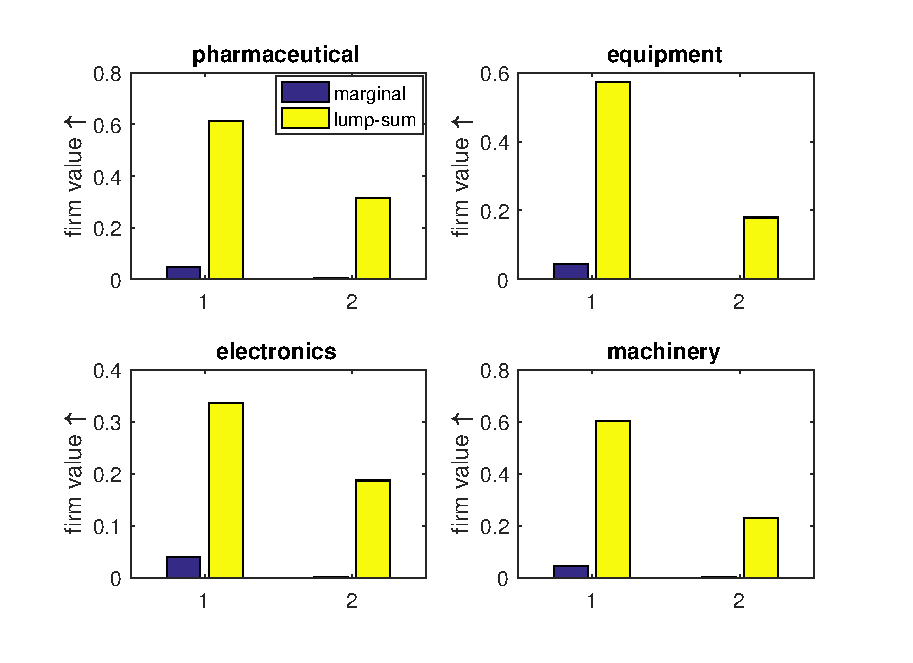
\includegraphics[width=\textwidth]{Figs/FirmvalueChange.eps}   
        \caption*{Panel A. Firm value}   
    \end{minipage}
     \hfill
     \begin{minipage}{0.48\textwidth}
         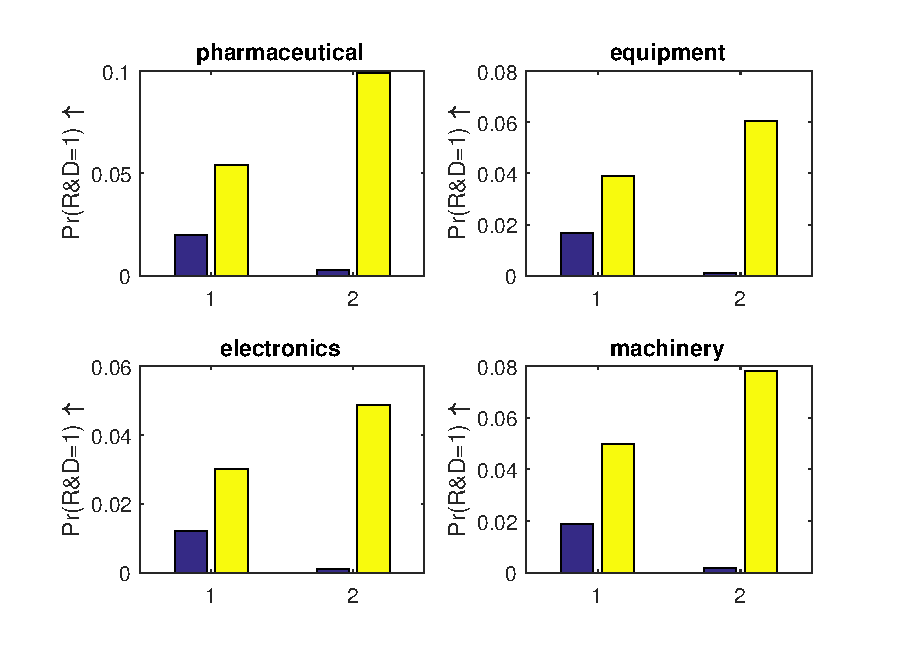
\includegraphics[width=\textwidth]{Figs/ProbChange.eps}
         \caption*{Panel B. Innovation prob.}
     \end{minipage}
    \caption*{\small{}Note: in all the graphs, '1' represents subsidy on the maintenance costs, '2' represents subsidy on the start-up costs. Firm value is measured in 10,000 US dollars.}{\small \par}
\end{figure}

Furthermore, we display the results on the impact of R\&D subsidy on innovation participation in Panel B of Figure \ref{F6}. Now the implication of the results becomes different. We have following important observations from the results. First, for all the industries, lump-sum subsidy is more effective than proportional subsidy. Second, different subsidy programs have different impact on increasing the innovation probability when implemented for different types of R\&D costs. For the proportional subsidy, reducing the maintenance costs is more effective in enhancing the probability of investing in R\&D. However, lump-sum subsidy is found to be more effective when financing the start-up costs of R\&D investment. Note that these results are dependent on the assumption of the distribution of R\&D costs as well as the distribution of the states. 

\textit{The effect of one unit R\&D subsidy.} To investigate the cost-benefit efficiency of R\&D subsidy, we further compute the increase in firm value and/or innovation participation caused by one unit expenditure on R\&D subsidy. The results are displayed in Figure \ref{F7} . We can find that: first, lump-sum subsidy is more efficient than proportional subsidy either for increasing the firm value of increasing the innovation participation. Second, subsidizing the maintenance costs is more efficient. It is worth mentioning that these counterfactual results depend on the the functional forms chosen in our structural model. However, they do show that lump-sum transfer works better by increasing the expected benefits of innovation uniformly. 

\begin{figure}[h]
    \caption{Impacts per unit R\&D subsidy: $\delta^m=0.80$}
    \label{F7}
    \centering
    \begin{minipage}{0.48\textwidth}
      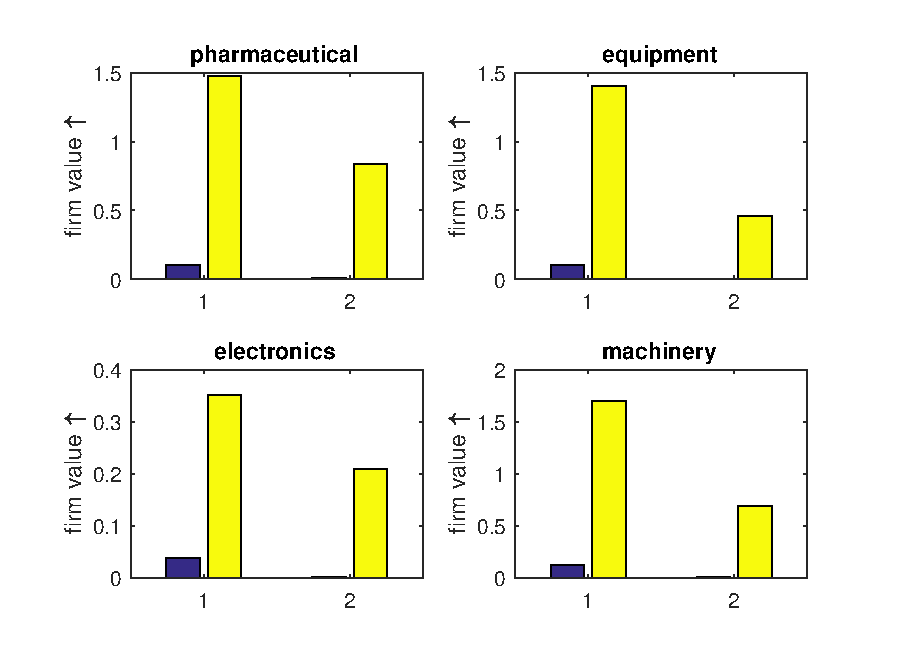
\includegraphics[width=\textwidth]{Figs/valuechangePerUnit.eps}  
      \caption*{Panel A. Firm value}      
    \end{minipage}
    \hfill
    \begin{minipage}{0.48\textwidth}
        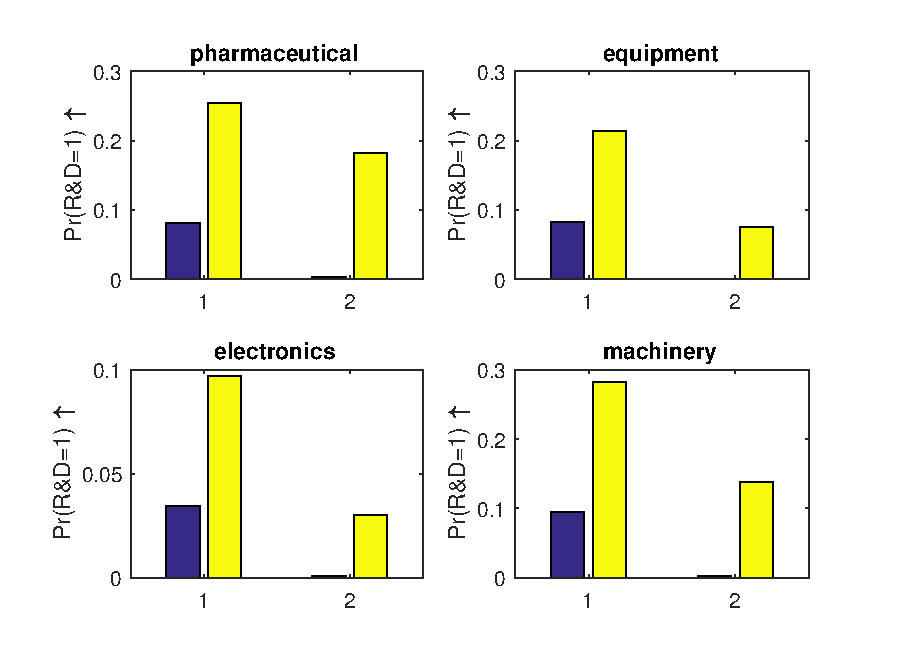
\includegraphics[width=\textwidth]{Figs/probchangePerUnit.eps}
        \caption*{Panel B. Innovation prob.}
    \end{minipage}
    \caption*{\small{}Note: in all the graphs, '1' represents subsidy on the maintenance costs, '2' represents subsidy on the start-up costs. Firm value is measured in 10,000 US dollars.}{\small \par}
    \end{figure}


\section{Conclusion}
Understanding the costs and benefits of R\&D investment is crucial for the designing of innovation policy in spurring R\&D investment. The benefits of R\&D are realized through different channels. Even in the presence of innovation failure, R\&D investment can still promote the firm's productivity through knowledge accumulation. Since it is hard to find a perfect measure for the innovation outcome, including R\&D in addition to innovation outcome in evaluating the benefits of innovation is necessary for obtaining more accurate estimates for the benefits of R\&D. 

By allowing a flexible relationship between innovation and productivity, this paper proposes an empirical framework to decompose the benefits of R\&D into patent and non-patent channels. The structural model extends an existing framework to incorporate both input and output of innovation into the evolution of productivity. Applying it to a sample of Chinese high-tech manufacturing firms, I find that Chinese high-tech firms generate much lower benefits from innovation than existing estimates of high-tech firms in Germany. More interestingly, most of the benefits of R\&D investment originates from non-patenting R\&D investment. The estimation framework also provides a new approach for estimating the value of patents. Based on the structural estimates, I perform a series of counterfactual analysis to evaluate the effectiveness of different R\&D subsidy schemes. Overall, the results suggest that lump-sum transfer is more efficient than the marginal subsidy. 



\clearpage 
\appendix 
\appendixpage 
\section{An Empirical Framework with Intensive-margin R\&D Investment}
In this section, I first briefly lay out an extended dynamic model with R\&D investment and patents. The basic structure of the model is similar to that considered in \cite{Awetal.2011,Doraszelski2013,Peters2016, Peters2017rand}, with the exception that both R\&D and patents play a role in shifting the future productivity. 

\subsection{A Model of R\&D Investment}

\paragraph{Production and Profits} A firm has a Cobb-Douglas production function
\begin{equation}
Q_{it} = \Phi_{it}K_{it}^{\beta_{k}}L_{it}^{\beta_l}M_{it}^{\beta_m}\exp{(\beta_a a_{it})}
\end{equation}
where $Q_{it}$ is the physical output of firm $i$ in period t, $\Phi_{it}$ is the total factor productivity, $K_{it}$ is the capital, $L_{it}$ is the labor, $M_{it}$ is the material, $a_{it}$ is the firm's age. Consider a well-behaved inverse demand equation
\begin{equation}
    p_{it} = D(Q_{it})
\end{equation}
where $p_{it}$ is the output price. To simplify the analysis, we assume that a firm treats capital and productivity as predetermined when choosing labor and materials in each period. Let $\Pi(\phi_{it},\mathbf{S}_{it})$ be the optimal profits, and $R(\phi_{it},\mathbf{S}_{it})$ be the revenue, where $\phi_{it}=\ln(\Phi_{it})$, $\mathbf{S}_{it}=(K_{it}, P_{Lit}, P_{Mit}, a_{it})$ is a vector of exogenous state variables. The cost minimization implies that
\begin{equation}
    \Pi(\phi_{it},\mathbf{S}_{it}) = (1-\frac{\beta_l+\beta_m}{\theta_{it}})R(\phi_{it},\mathbf{S}_{it})
\end{equation}
where $\theta_{it}$ is the markup. Note that when $\beta_l+\beta_m=1$, the production function is of constant return to scale in terms of $L_{it}$ and $M_{it}$.

\paragraph{Productivity evolution}The firm's productivity $\phi_{it}$ is unobserved by the econometrician. R\&D investment and patenting enter the Markov process governing the productivity evolution. In particular, the dynamics of the productivity is given by
\begin{equation}
    \phi_{it+1} = h(\phi_{it},d_{it},\mathbf{o}_{it+1})+\epsilon_{it+1}
\end{equation}
where $d_{it}$ represents the R\&D investment and $\mathbf{o}_{it+1}$ is a vector summarizing the innovation outcome next period, and $\epsilon_{it+1}$ is an iid shock with a mean-zero normal distribution. Considering different types of innovation output, $\mathbf{o}_{it}$ can be a vector of process innovation and product innovation measured by the patents or other observed indicators. The marginal effects of R\&D investment and innovation output are captured by three partial derivatives $\partial h/\partial d_{it}$, $\partial h/\partial \mathbf{o}_{it+1}$, and a cross derivative $\partial ^2h/\partial d_{it} \partial \mathbf{o}_{it+1}$. Because R\&D is the fundamental source of productivity change, we impose that $ \partial h(\phi_{it}, 0, \mathbf{o}_{it+1})/\partial\mathbf{o}_{it+1} = \mathbf{0}$. This implies that without R\&D investment, we should expect no endogenous productivity growth, though we can see productivity growth through the channel of exogenous shocks. The cross-derivative $\partial ^2h/\partial d_{it} \partial \mathbf{o}_{it+1}$ deserves some discussion. When positive, it means that the stimulating impact of R\&D on productivity is strengthened through the patenting. This indicates that the patenting system help firms protect their inventions. When negative, we anticipate that the effect of knowledge spillovers dominates so that firms productivity improves less by patenting. This may be due to the weak patenting system.

Following CDM, I assume that patents is a random variable of which the distribution is determined by R\&D investment. This assumption greatly simplifies the analysis by only considering the R\&D investment choice. Specifically, patents outcome in next period is assumed to be a distribution depending on past R\&D. The distribution of $\mathbf{o}_{it+1}$ is given by $Pr(\mathbf{o}_{it}\leq \mathbf{o}) = G(\mathbf{o};d_{it})$.\footnote{In the reduce-form analysis, this process is usually estimated using count data models. See \cite{hall1989research,hall2010handbook}.} This layer of uncertainty is similar to that considered in PRVF. Note the Markovian property implies that the conditional expectation of future productivity is 

\begin{equation*}
    \mathbf{E}(\phi_{it+1}|\phi_{it}, d_{it})=\int h(\phi_{it},d_{it},\mathbf{o})dG(\mathbf{o};d_{it})
\end{equation*}
Therefore R\&D investment can influence future productivity through affecting $h(\phi_{it}, d_{it},\mathbf{o})$ and the distribution of innovation output $G(\mathbf{o}; d_{it})$. This allows me to decompose the impact of R\&D into patenting and non-patenting channels.


\paragraph{Recursive formulation}
To consider a general setting, denote $C(d_{it}, \mathbf{X}_{it})$ as the variable costs of R\&D investment. Here $\mathbf{X}_{it}=(\mathbf{S}_{it}, \mathbf{Z}_{it})$, $\mathbf{Z}_{it}$ is the additional exogenous states that influence the costs of R\&D investment.\footnote{For example, $\mathbf{Z}_{it}$ may contain past R\&D investment decisions so the R\&D costs also include adjustment costs.} In addition, there is a fixed cost of R\&D investment, denoted as $f(\mathbf{X}_{it})$. With this fixed costs, the model can capture the innovation choice at the extensive margin. Note that we allow the exogenous state variables to affect the costs of R\&D. Omitting the subscripts, the firm's dynamic programming problem can be written in a recursive formulation:
\begin{equation}\label{VF_full}
    V(\phi, \mathbf{X}) =\max_{d}\left\{V^0(\phi, \mathbf{X}), V^d(\phi, \mathbf{X})\right\} 
\end{equation}
where the value functions for different choices of $d$ are
\begin{align}
    V^0(\phi)&=\Pi(\phi,\mathbf{X})+ \beta \mathbf{E}\left[ V(\phi', \mathbf{X}')|d=0\right], \\
    V^d(\phi)&=\max_{d} \left\{ \Pi(\phi,\mathbf{X})-C(d, \mathbf{X}) - f(\mathbf{X}) + \beta \mathbf{E}\left[ V(\phi', \mathbf{X}')|d\right]\right\}, \label{VF_d}
\end{align}
where $\beta$ is the discounting factor. We assume that firms have perfect foresight for the exogenous state variables. This allows us to calculate the expected firm value as
\begin{equation}\label{EV_d}
    \mathbf{E}\left[ V(\phi', \mathbf{X}')|d\right] = \int\int V(h(\phi,d,\mathbf{o})+\epsilon,\mathbf{X}')dG(\mathbf{o};d)dF(\epsilon)
\end{equation}
where $F(\cdot)$ is the distribution of $\epsilon'$. 
A stochastic equilibrium of the model is a decision rule $d(\phi, \mathbf{X})\geq0$ such that the recursive problem (\ref{VF_full}) is solved.

\section{Math Derivations} \label{app_revenue_equation}
\subsection*{Profit maximization and revenue equation} \label{app_revenue_equation}
The firm's profits maximization problem is
\begin{align*}
\max_{L_{it},\,M_{it}} & \left\{ P_{it}Q_{it}-P_{Lt}L_{it}-P_{Mt}M_{it}\right\} \\
s.t.\, & Q_{it}=P_{it}^{-\sigma}P_{t}^{\sigma}Q_{t}\\
 & Q_{it}=\Phi_{it}K_{it}^{\beta_{k}}L_{it}^{\beta_{l}}M_{it}^{\beta_{m}}\exp\left(\beta_{a}a_{it}\right)
\end{align*}
Write the revenue as a function of the output, the first-order conditions
are:
\begin{align}
\left(1-\frac{1}{\sigma}\right)\left(P_{t}^{\sigma}Q_{t}\right)^{\frac{1}{\sigma}}Q_{it}^{-\frac{1}{\sigma}}\frac{\partial Q_{it}}{\partial L_{it}} & =P_{Lt}\\
\left(1-\frac{1}{\sigma}\right)\left(P_{t}^{\sigma}Q_{t}\right)^{\frac{1}{\sigma}}Q_{it}^{-\frac{1}{\sigma}}\frac{\partial Q_{it}}{\partial M_{it}} & =P_{Mt}
\end{align}
where $\frac{\partial Q_{it}}{\partial M_{it}}=\beta_{m}\frac{Q_{it}}{M_{it}}$
and $\frac{\partial Q_{it}}{\partial L_{it}}=\beta_{l}\frac{Q_{it}}{L_{it}}$.
This implies that 
\begin{equation}
M_{it}=\frac{P_{Lt}}{P_{Mt}}\frac{\beta_{m}}{\beta_{l}}L_{it}
\end{equation}
Plugging this back to the foc for $L_{it}$, we obtain
\begin{align}
P_{Lt} & =\beta_{l}\left(1-\frac{1}{\sigma}\right)\left(P_{t}^{\sigma}Q_{t}\right)^{\frac{1}{\sigma}}\frac{Q_{it}^{1-\frac{1}{\sigma}}}{L_{it}}\nonumber \\
 & =\beta_{l}\left(1-\frac{1}{\sigma}\right)\left(P_{t}^{\sigma}Q_{t}\right)^{\frac{1}{\sigma}}\left(\frac{P_{Lt}}{P_{Mt}}\frac{\beta_{m}}{\beta_{l}}\right)^{\frac{\beta_{m}\left(\sigma-1\right)}{\sigma}}\left(\Phi_{it}K_{it}^{\beta_{k}}e^{\beta_{a}a_{it}}\right)^{1-\frac{1}{\sigma}}L_{it}^{\frac{\left(\beta_{l}+\beta_{m}\right)\left(\sigma-1\right)}{\sigma}-1}\nonumber \\
\Rightarrow\:L_{it} & =\left[\frac{P_{Lt}\left(\frac{P_{Lt}}{P_{Mt}}\frac{\beta_{m}}{\beta_{l}}\right)^{\frac{\beta_{m}\left(1-\sigma\right)}{\sigma}}}{\beta_{l}\left(1-\frac{1}{\sigma}\right)\left(P_{t}^{\sigma}Q_{t}\right)^{\frac{1}{\sigma}}}\left(\Phi_{it}K_{it}^{\beta_{k}}\exp\left(\beta_{a}a_{it}\right)\right)^{\frac{1-\sigma}{\sigma}}\right]^{\frac{\sigma}{\left(\beta_{l}+\beta_{m}\right)\left(\sigma-1\right)-\sigma}}
\end{align}
Also note that the foc for $L_{it}$ also implies that the revenue
can be expressed as
\begin{equation}
R_{it}=\frac{\sigma P_{Lt}L_{it}}{\beta_{l}\left(\sigma-1\right)}
\end{equation}
 When $\beta_{l}+\beta_{m}=1$, combining these two expressions and
take logs yields:
\begin{equation}
r_{it}=\mu_{0}+\mu_{t}+\left(\sigma-1\right)\left(\beta_{k}k_{it}+\beta_{a}a_{it}+\phi_{it}\right)
\end{equation}
where 
\begin{align}
\mu_{0} & =\left(\sigma-1\right)\ln\left(\frac{\sigma-1}{\sigma}\beta_{l}^{\beta_{l}}\beta_{m}^{\beta_{m}}\right)\\
\mu_{t} & =\left(1-\sigma\right)\ln\left(P_{Lt}^{\beta_{l}}P_{Mt}^{\beta_{m}}\right)+\ln\left(P_{t}^{\sigma}Q_{t}\right)
\end{align}

\section{Supplementary Results}
\subsection{Data features} \label{app_data_features}
In this appendix, I present more features of the
data for Chinese high-tech manufacturing firms. In particular, I will discuss the distributional characteristics for patents and the R\&D-patents relation. These discussions suggest that the extensive margins of R\&D and patents captures most part of the innovation activities. 

\textit{Distribution of patents.} Table \ref{T3} reports the distribution of patents. We can see that
the distribution of patents is highly concentrated at zero for all
three types of patents. The share of firm observations
with zero invention (utility) patents in the final sample is 98.01\%
(95.72\%). This implies that only a small fraction of firms file
patent applications. Focusing on the positive part of the distribution,
the percentage of firm observations filing only one invention (utility)
patent is 1.22\% (2.22\%), and that of firm observations filing two
invention (utility) patents is 0.39\% (0.96\%). Moreover, the number
of firm observations submitting no less than three invention (utility)
patents account for 0.37\% (1.10\%) in the sample. Overall,
these observations imply that the variation in the patents outcome
in positive part (extensive margin) is much less significant than
the change from zero to one (i.e. the extensive margin) for invention
and utility patents. In other wods, among firms that have positive
patent applications, most of the firms (over 50\%) have only one patents. Overall, these results suggest that we have to rely on the variation in extensive margin to identify the productivity effects of the patents.

\begin{table}[h]
\centering
\caption{Distribution of patents for high-tech manufacturing firms}
\label{T3}
\begin{tabular}{lccccc}
\toprule
Patents counts & 0       & $\geq 1$ & 1      & 2      & $\geq 3$ \\
\hline
Invention&98.01\% & 1.99\% & 1.22\% & 0.39\% & 0.37\% \\
Utility&95.72\% & 4.28\% & 2.22\% & 0.96\% & 1.10\% \\ \bottomrule
\end{tabular}

{\small{}Note:the percentage represents the share of observations in the specified cohort.}{\small \par}
\end{table}

\textit{R\&D-patents relation.} The R\&D-patents linkage is an important part in the structural model to be explained in next section. Since I do not have a direct measure for innovation, I rely on the patents to measure the outcome of innovation. Different from the indicators of process and product innovation used in PRVF, I observe the number of invention patents and/or utility patents filed by each firm. To check the validity of using patents as indicators for innovation, I report the correlation between patents and R\&D at both intensive and extensive margins in Table \ref{T4}. I estimate a linear model relating patents applications to R\&D investment controlling for industry, and year fixed effects. I also control for firm size by use R\&D intensity defined as the ratio of R\&D expenditures to firm's sales. 

\begin{table}[h]
\centering
\caption{Correlation between different margins of R\&D and patents}
\label{T4}
\begin{tabular}{cllllll}
\toprule
 & \multicolumn{3}{c}{invention patents} & \multicolumn{3}{c}{utility patents} \\
 margins& extensive   & intensive  & both       & extensive  & intensive  & both      \\
                                          \hline 
\multirow{2}{*}{extensive} & .0402***   & -.216     & .0732***  & .0444***  & .165      & .121***  \\
                                          & (.003)     & (.284)    & (.009)    & (.003)    & (.374)    & (.025)   \\
                                          \hline
\multirow{2}{*}{intensive} & 0.690***    & 3.214      & 1.631***   & .403***   & 3.319      & 1.350**   \\
                                          & (.120)     & (2.196)    & (.364)    & (.109)    & (3.060)    & (.442)   \\
 \hline
\multirow{2}{*}{both}                     & .883***   & 1.015      & 1.883***   & .780***  & 2.870      & 2.302***  \\
                                          & (.110)     & (2.497)    & (.327)    & (.107)    & (3.109)    & (.476)  \\ \bottomrule
\end{tabular}
\caption*{\small{}Note: all regression contain industry and year fixed effects. Results in columns (1) and (3) are obtained using all the sample; columns (2) and (4) display the results using observations with positive patent applications. Standad errors are in parentheses. * \(p<0.05\), ** \(p<0.01\), *** \(p<0.001\)} {\small \par}
\end{table}


The matrix of regression coefficients in Table \ref{T4} show that only the correlation between the extensive margin of invention patents and R\&D investment is positive and highly significant. This implies that the variation in patents outcome at the intensive margin is not well explained by the firm's R\&D effort. Because R\&D is the fundamental source of innovation, we will expect that the variation in patents along the intensive margin will not have significant impact on firm's growth. Another important observation from the table is that the intensive margin of R\&D is an important explanatory variable for the extensive margin of patents outcome. However, the correlation coefficient becomes much larger if we consider both margins of R\&D and use R\&D intensity as the indicator for R\&D. This suggests that the change of R\&D from zero to positive has much larger marginal impact in generating patents. In the data, the fraction of firms with zero patent is around 30\%, while the fraction is increased to be 60\% for firms with at least one invention or utility patent. In contrast, the mean value of R\&D for firms with at least one patent is only slightly higher than firms without any patent. This confirms that the variation in R\&D along the extensive margin is the main driver in explaining the patents outcome. 

\begin{table}[h]

    \centering
    \caption{Estimates of productivity evolution equation: supplementary results}
    \label{TA}
    {
\def\sym#1{\ifmmode^{#1}\else\(^{#1}\)\fi}
\begin{tabular}{l*{1}{cc}}
\toprule
\multicolumn{3}{c}{productivity evolution equation  }\\
\midrule  
$\omega_t$       &       0.826\sym{**}&     (17.13)\\
$\omega_t^2$     &        0.300\sym{**}&     (15.87)\\

$rd_t$    &     0.00505\sym{**}&      (3.35)\\

$rd_t\times n_{t+1}$      &      0.0153\sym{**}&      (3.04)\\
$rd_t \times b_{t+1}$      &     0.0142\sym{*} &      (2.85)\\
$\beta_k$                  & -0.308\sym{**}    &     (-25.71)\\
\midrule
\(N\)       &       22492        &            \\
\bottomrule
\end{tabular}
}

    \caption*{\small{}Note:T statistics are in parentheses; {*} p$<$0.05, {*}{*}
    p$<$0.01. }{\small \par}
    \end{table}
    

\subsection{NLLS estimation} \label{appc2}
As a robustness check, we also try to parameterize $h(\cdot)$ as a quadratic function. The estimation results are reported in Table \ref{TA}. In order to use the first-stage estimates to calculate the value function, we need to check the first-order derivative of $h(\cdot)$ with respect to $\phi_{it}$. To ensure that firms have some incentives to invest in R\&D and their value functions are bounded, we require this derivative is between 0 and 1. In figure \ref{F2}, we show the empirical $\partial h(\cdot)/\partial\phi_t$ against productivity for different forms of $h$. It is clear that the quadratic form would provide a poor prediction of R\&D investment in the data because the non-stationary productivity process will discourage firms from undertaking R\&D investment in the infinite-horizon model. 
\begin{figure}[h]
  \centering
  \caption{First-order derivative of $h(\cdot)$ with respect to $\phi_{it}$}
  \label{F2}
  \begin{minipage}[b]{0.45\textwidth}
    \caption*{Panel A: Cubic form}
    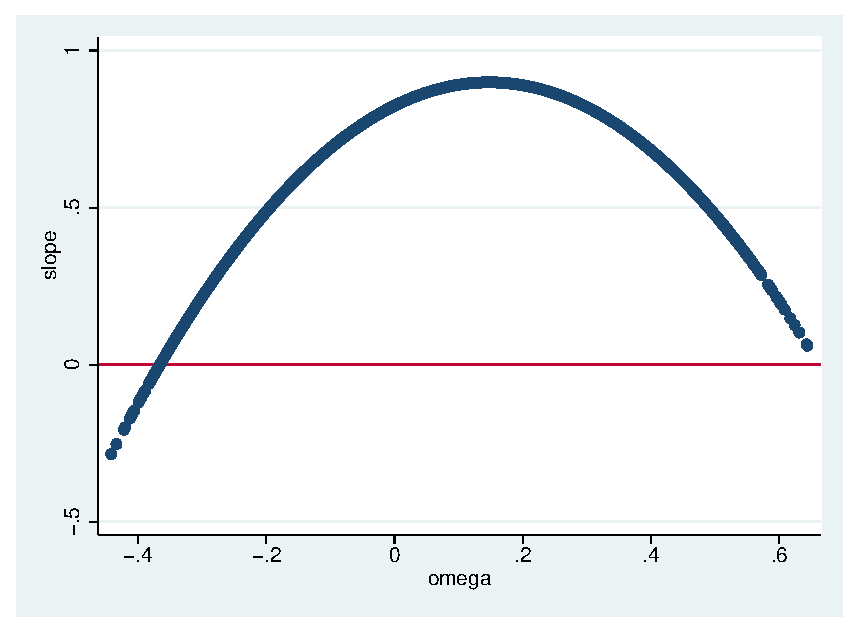
\includegraphics[width=\textwidth]{Figs/slope_benchmark.eps}\label{slope1_fig}
  \end{minipage}
  \hfill 
  \begin{minipage}[b]{0.45\textwidth}
    \caption*{Panel B: Quadratic form}
    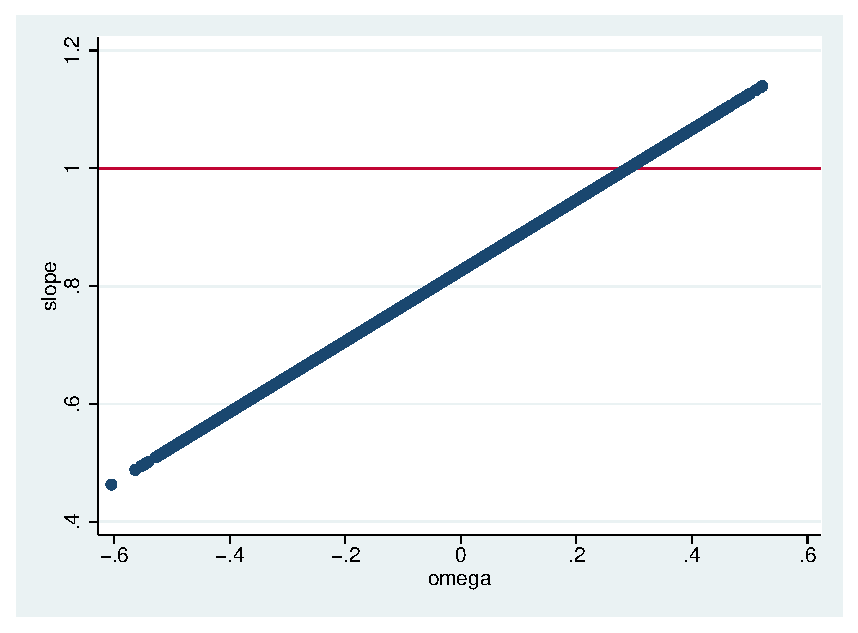
\includegraphics[width=\textwidth]{Figs/slope_robustness.eps}
  \end{minipage}
 \caption*{Note: in the cubic form, the number of observations that has the slope below zero is 89; in the quadratic equation,the number of observations with slope greater than one is 517. }
\end{figure}
\subsection{Computation} \label{app_comp}
\subsubsection{Discretizing non-linear Markov process}

For this part, I refer to Farmer and Toda (2017). 

\subsubsection{Nested fixed point algorithm}

\paragraph{Profit function}

I normalize the productivity with the constant $\psi_{0}$ in the
empirical model. From the estimation equation, we can write the profit
as:
\begin{equation}
\hat{r}_{it}\left(\hat{\omega}_{it}\right)=\hat{\psi}_{0}+\hat{\psi}_{t}+\left(1+\hat{\theta}_{j}\right)\hat{\rho}_{0}+\left(1+\hat{\theta}_{j}\right)\hat{\beta}_{k}k_{it}+\left(1+\hat{\theta}_{j}\right)\hat{\beta}_{a}a_{it}-\left(1+\hat{\theta}_{j}\right)\hat{\omega}_{it}
\end{equation}
It follows that the profit can be calculated as 
\begin{equation}
\pi_{it}\left(\hat{\omega}_{it}\right)=-\frac{1}{\hat{\theta}_{j}}\exp\left(\hat{r}_{it}\left(\hat{\omega}_{it}\right)\right)
\end{equation}

\paragraph{Choose the grid points}

We perform the computation by industry. Several coefficients are specific
to each industry: $\psi_{0}$, $\rho_{0}$, and $\theta_{j}$. Note
that we discretize the productivity into 200 grid points, and age
into 4 groups. To implement the estimation, I use the trapezoid method
to discretize the capital space in evenly distributed 100 points.
Therefore, we are encountered with $100\times4\times4=1600$ types
of firms. For each type of firm, we solve the value function for $100\times2=200$
states. In the end, we solve $1600\times200=320000$ value functions.
We compute the value function by industry by industry. 

\paragraph{Inner loop: Value function iteration}

Given $\left(\omega_{it},\,k_{it},\,a_{it}\right),$ we use $V_{d}$
to denote $V\left(\omega_{it},rd_{it-1}=d;\,k_{it},a_{it}\right)$.
We also define $\gamma_{it}^{d}\equiv\gamma_{it}\left(rd_{it-1}=d,k_{it};\,\kappa^{m},\,\kappa^{s}\right)$,
for $d\in\left\{ 0,\,1\right\} $, and $\kappa\equiv\left(\kappa^{s},\,\kappa^{m}\right)$
be the parameter to be estimated. Employing the exponential distribution,
we can express the value function as 
\begin{align*}
V_{d} & =\pi_{it}\left(\omega_{it}\right)+\beta\int_{0}^{\Delta EV}\left(EV_{1}-\tau\right)dG\left(\tau\right)+\beta\int_{\Delta EV}^{\infty}EV{}_{0}dG\left(\tau\right)\\
 & =\pi_{it}\left(\omega_{it}\right)+\beta EV_{1}\left(1-e^{-\frac{\Delta\mathbb{E}V}{\gamma_{it}^{d}}}\right)+\beta\left(\Delta EV+\gamma_{it}^{d}\right)e^{-\frac{\Delta\mathbb{E}V}{\gamma_{it}^{d}}}\\
 & -\beta\gamma_{it}^{d}+\beta EV{}_{0}e^{-\frac{\Delta\mathbb{E}V}{\gamma_{it}^{d}}}
\end{align*}
where $\Delta EV=EV_{1}-EV_{0}$. Therefore the expression of $V_{d}$
can be simplified as 
\begin{equation}
V_{d}=\pi_{it}\left(\omega_{it}\right)+\beta\gamma_{it}^{d}\left(\exp\left(-\frac{\Delta EV}{\gamma_{it}^{d}}\right)-1\right)+\beta EV_{1},\,\text{for }d\in\left\{ 0,\,1\right\} \label{Vd}
\end{equation}
In computing the value functions, $V_{d}$ is a $200$ by 1 vector
given capital, age, and industry. Let $p_{mn}=Pr\left(n_{t+1}=m,b_{t+1}=n|rd_{t}=1\right)$,
for $m,\,n\in\left\{ 0,1\right\} $, and further denote $P_{mn}$
as the corresponding transition matrix of the productivity and $P_{0}$
as the transition matrix of productivity when $rd_{t}=0$. then Equation
(\ref{Vd}) can be transformed as 
\begin{align}
V_{1} & =\pi\left(\omega\right)-\beta\gamma^{1}\left(1-\exp\left(-\frac{\Delta EV}{\gamma^{1}}\right)\right)+\beta\left(\sum_{m}\sum_{n}p_{mn}P_{mn}\right)V_{1}\label{V1}\\
V_{0} & =\pi\left(\omega\right)-\beta\gamma^{0}\left(1-\exp\left(-\frac{\Delta EV}{\gamma^{0}}\right)\right)+\beta\left(\sum_{m}\sum_{n}p_{mn}P_{mn}\right)V_{1}\label{V0}
\end{align}
Denote $P_{1}=\beta\left(\sum_{m}\sum_{n}p_{mn}P_{mn}\right)$, then
\[
V_{1}=\left(I-\beta P_{1}\right)^{-1}\left[\pi\left(\omega\right)-\beta\gamma^{1}\left(1-\exp\left(-\frac{\Delta EV}{\gamma^{1}}\right)\right)\right]
\]
 because $\Delta EV=P_{1}V_{1}-P_{0}V_{0}$, it follows that:
\begin{align}
\Delta EV & =\left(I-\beta P_{0}\right)P_{1}\left(I-\beta P_{1}\right)^{-1}\left[\pi\left(\omega\right)-\beta\gamma^{1}\left(1-\exp\left(-\frac{\Delta EV}{\gamma^{1}}\right)\right)\right]\label{DEV}\\
 & \quad-P_{0}\left[\pi\left(\omega\right)-\beta\gamma^{0}\left(1-\exp\left(-\frac{\Delta EV}{\gamma^{0}}\right)\right)\right]\nonumber 
\end{align}
We use equation (\ref{DEV}) to solve for $\Delta EV$ and then we
use equations (\ref{V1}) and (\ref{V0}) to solve for $V_{1}$ and
$V_{0}$. Use $T_{\kappa}$ as the linear operator applied to $\Delta EV$,
it is easy to show that $T_{\kappa}$ is a contraction mapping. Then
$\Delta EV$ is a fixed point such that 
\[
T_{\kappa}\left(\Delta EV\right)=\Delta EV
\]
.Now we are in the position to use Newton-Kantorovich iterations.
First note that the Frech\'{e}t derivative of $T_{\kappa}$ with
respect to $\Delta EV$ is:
\begin{align}
T_{\kappa}' & =\frac{\partial T_{\kappa}\left(\Delta EV\right)}{\partial\Delta EV}\\
 & =\beta\left(\beta P_{0}-I\right)P_{1}\left(I-\beta P_{1}\right)^{-1}\exp\left[\text{diag}\left\{ -\frac{\Delta EV_{i}}{\gamma^{1}}\right\} \right]\nonumber \\
 & +\beta P_{0}\exp\left[\text{diag}\left\{ -\frac{\Delta EV_{i}}{\gamma^{0}}\right\} \right]\nonumber 
\end{align}
where 
\[
\text{diag}\left\{ -\frac{\Delta EV_{i}}{\gamma^{d}}\right\} =\left[\begin{array}{cccc}
-\frac{\Delta EV_{1}}{\gamma^{d}} & 0 & \cdots & 0\\
0 & -\frac{\Delta EV_{2}}{\gamma^{d}} & \cdots & 0\\
\vdots & \vdots & \ddots & \vdots\\
0 & 0 & \cdots & -\frac{\Delta EV_{n}}{\gamma^{d}}
\end{array}\right]
\]
Using the invertibility of $\left[I-T_{\kappa}'\right]$ the $n$th
iteration in the Newton-Kantorovich algorithm is 
\[
\Delta EV_{n+1}=\Delta EV_{n}-\left[I-T_{\kappa}'\right]^{-1}\left(I-T_{\kappa}\right)\left(\Delta EV_{n}\right)
\]
We set the tolerance as $e^{-6}$; the iteration stops when $\|\Delta EV_{n+1}-\Delta EV_{n}\|\leq e^{-6}$. 

\paragraph{Outer loop: BHHH optimization algorithm}

The outer loop solves following problem:
\[
\max_{\kappa^{s},\kappa^{m}}\sum_{i}\sum_{t}l_{it}\left(\kappa,\,\Delta EV_{it}\right)
\]
 where 
\begin{align}
l_{it}\left(\kappa,\,\Delta EV_{it}\right) & =\log\left\{ rd_{it}Pr\left(rd_{it}=1|\kappa,rd_{it-1}\right)+\left(1-rd_{it}\right)Pr\left(rd_{it}=0|\kappa,rd_{it-1}\right)\right\} \label{llf}\\
 & =\log\left\{ \left(2rd_{it}-1\right)\Pr\left(rd_{it}=1|\kappa,rd_{it-1}\right)+1-rd_{it}\right\} \nonumber 
\end{align}
where $\Delta EV_{it}=\Delta EV\left(\omega_{it}\right)$ and 
\begin{align}
Pr\left(rd_{it}=0|\kappa,rd_{it-1}\right) & =1-Pr\left(rd_{it}=1|\kappa,rd_{it-1}\right)\\
 & =\exp\left\{ \frac{-\beta\Delta EV\left(\omega_{it}\right)}{\kappa^{m}rd_{it-1}k_{it}+\kappa^{s}\left(1-rd_{it-1}\right)k_{it}}\right\} \nonumber 
\end{align}
The basic parameter iteration under BHHH algorithm is:
\begin{align*}
\kappa_{n+1} & =\kappa_{n}+\lambda\underset{\equiv D\left(\kappa_{n}\right)}{\underbrace{\left[\sum_{i,t}\left(\frac{\partial l_{it}\left(\kappa_{n},\,\Delta EV_{it}\right)}{\partial\kappa_{n}}\right)\left(\frac{\partial l_{it}\left(\kappa_{n},\,\Delta EV_{it}\right)}{\partial\kappa_{n}'}\right)\right]^{-1}\left(\sum_{i,t}\frac{\partial l_{it}\left(\kappa_{n},\,\Delta\right)}{\partial\kappa_{n}}\right)}}
\end{align*}
From (\ref{llf}) we know that 
\begin{equation}
\frac{\partial l_{it}\left(\kappa_{n},\,\Delta EV_{it}\right)}{\partial\kappa_{n}'}=w_{it}\left[\frac{\partial Pr\left(rd_{it}=1|\kappa,rd_{it-1}\right)}{\partial\kappa_{n}^{s}},\,\frac{\partial Pr\left(rd_{it}=1|\kappa,rd_{it-1}\right)}{\partial\kappa_{n}^{m}}\right]
\end{equation}
where
\begin{align*}
w_{it} & =\frac{\left(2rd_{it}-1\right)}{\left(2rd_{it}-1\right)\Pr\left(rd_{it}=1|\kappa,rd_{it-1}\right)+1-rd_{it}}\\
\frac{\partial Pr\left(rd_{it}=1|\kappa,rd_{it-1}\right)}{\partial\kappa_{n}^{s}} & =\beta\frac{\frac{\partial\Delta EV_{it}}{\partial\kappa_{n}^{s}}\gamma_{it}^{rd_{it-1}}-\left(1-rd_{it-1}\right)k_{it}\Delta EV_{it}}{\left(\gamma_{it}^{rd_{it-1}}\right)^{2}\exp\left(\frac{\beta\Delta EV_{it}}{\gamma_{it}^{rd_{it-1}}}\right)}\\
\frac{\partial Pr\left(rd_{it}=1|\kappa,rd_{it-1}\right)}{\partial\kappa_{n}^{m}} & =\beta\frac{\frac{\partial\Delta EV_{it}}{\partial\kappa_{n}^{m}}\gamma_{it}^{rd_{it-1}}-rd_{it-1}k_{it}\Delta EV_{it}}{\left(\gamma_{it}^{rd_{it-1}}\right)^{2}\exp\left(\frac{\beta\Delta EV_{it}}{\gamma_{it}^{rd_{it-1}}}\right)}
\end{align*}
where $\frac{\partial\Delta EV_{it}}{\partial\kappa^{s}}$ ($\frac{\partial\Delta EV_{it}}{\partial\kappa^{m}}$)
is the element in 1st (2nd) column such that the corresponding productivity
in the row is $\omega_{it}$. To finish the nested fixed point algorithm,
we need to compute the derivatives of the expected value function,
$\partial\Delta EV/\partial\gamma$. Applying the implicit theorem
to $T_{\kappa}\left(\Delta EV\right)=\Delta EV$, we get 
\[
\frac{\partial\Delta EV}{\partial\kappa}=\left[I-T_{\kappa}'\right]^{-1}\frac{\partial T_{\kappa}\left(\Delta EV\right)}{\partial\kappa}
\]
From (\ref{DEV}), we know that 
\begin{align*}
\frac{\partial T_{\kappa}\left(\Delta EV\right)}{\partial\kappa} & =\left[\begin{array}{cc}
\frac{\partial T_{\kappa}\left(\Delta EV\right)}{\partial\kappa^{s}} & ,\frac{\partial T_{\kappa}\left(\Delta EV\right)}{\partial\kappa^{m}}\end{array}\right]
\end{align*}
where 
\begin{align*}
\frac{\partial T_{\kappa}\left(\Delta EV\right)}{\partial\kappa^{m}} & =\beta k\left(\beta P_{0}-I\right)P_{1}\left(I-\beta P_{1}\right)^{-1}\left[1-\exp\left(\frac{-\Delta EV}{\gamma^{1}}\right)-\frac{\Delta EV}{\gamma^{1}}\varodot\exp\left(\frac{-\Delta EV}{\gamma^{1}}\right)\right]\\ 
\frac{\partial T_{\kappa}\left(\Delta EV\right)}{\partial\kappa^{s}} & =\beta kP_{0}\left[1-\exp\left(\frac{-\Delta EV}{\gamma^{0}}\right)-\frac{\Delta EV}{\gamma^{0}}\varodot\exp\left(\frac{-\Delta EV}{\gamma^{0}}\right)\right]
\end{align*}
are both $200$-by-$1$ vectors and $k$ is the exogenous state variable:
capital stock. We use $\varodot$ to denote the element-wise product.
To determine the step size $\lambda,$ we use secant iteration to
find the solution to $\partial f\left(\lambda\right)/\partial\kappa=0$,
where $f\left(\lambda\right)\equiv L\left(\kappa+\lambda D\left(\kappa\right)\right)$.
The iteration is given as:
\begin{equation}
\lambda_{m+1}=\lambda_{m}-\frac{\left(\lambda_{m}-\lambda_{m-1}\right)f'\left(\lambda_{m}\right)}{f'\left(\lambda_{m}\right)-f'\left(\lambda_{m-1}\right)}
\end{equation}
where 
\begin{equation}
f'\left(\lambda_{m}\right)=\sum_{i,t}\frac{\partial l_{it}\left(\kappa+\lambda_{m}D\left(\kappa_{n}\right),\,\Delta EV_{it}\right)}{\partial\kappa'}D\left(\kappa_{n}\right)
\end{equation}
This iteration determines the optimal step size $\lambda^{*}$. Finally,
the iteration stops when $\|\kappa_{n+1}-\kappa_{n}\|\leq e^{-6}$. 

\subsection{Model fit} \label{app_model_fit}
\subsubsection{Predicted revenues} In Figure \ref{F3}, I present a scatter plot to check the relationship between the model predicted revenue and the revenue information in the data. We can see that the predicted revenues concentrates around the 45-degree line, which indicates the revenue equation fits the data well. 

\begin{center}
\begin{figure}[h]
\caption{Model fitness for the revenue data}
\label{F3}
\begin{centering}
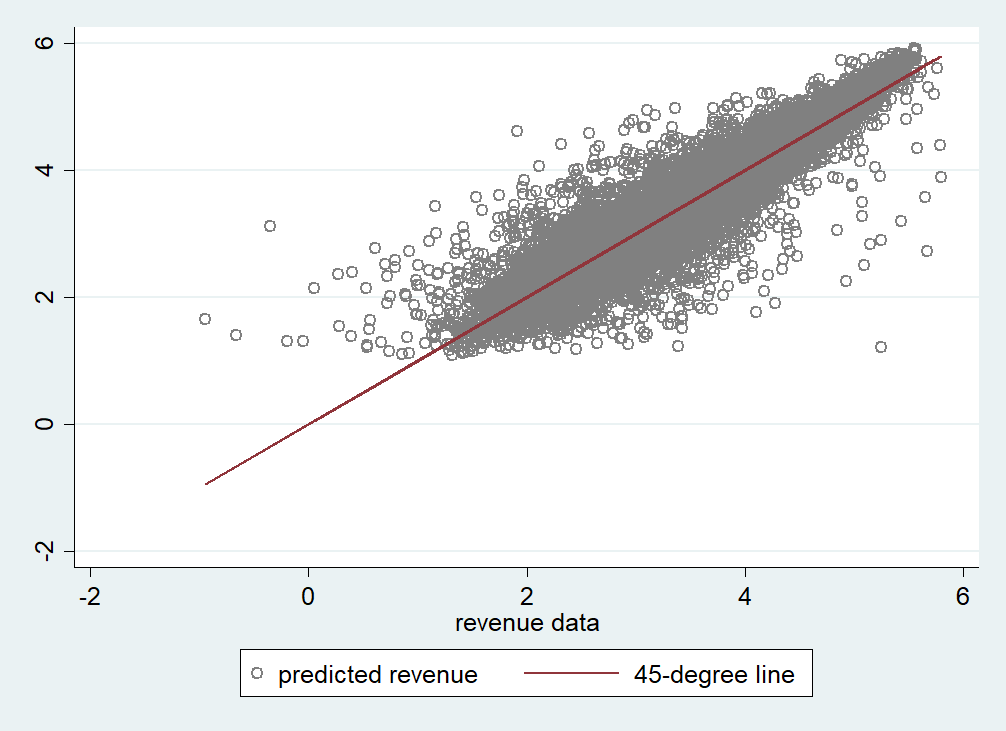
\includegraphics[width=0.7\textwidth]{Figs/revenue.png}
\par\end{centering}
\caption*{\small{}Note: sales are in logs of revenues in 100,000 USD.}{\small \par}
\end{figure}
\par\end{center}

\subsubsection{Pooled probability of investing in R\&D}
Given current state, we can solve for the probability of undertaking R\&D,$Pr(d=1|\phi,d_{-1},\mathbf{S})$ using equation (\ref{p_d}). Therefore the aggregate hazad function for R\&D choice can be calculated as:
\begin{equation}\label{hazad}
\mathcal{H}=\frac{1}{NT}\sum_{i}^{N}\sum_{t}^{T} Pr(d_{it}=1|\phi_{it},d_{it-1},\mathbf{S}_{it})
\end{equation}
On the other hand, in the data the probability of investing in R\&D is given as
\begin{equation}
\tilde {\mathcal{H}}=\frac{1}{NT}\sum_{i}^{N}\sum_{t}^{T} d_{it}
\end{equation}
I calculate the hazad function for each sector. The results are displayed in Table \ref{T15}. Overall, the estimated model predicts the probability of innovation similar to that exhibited in the data. The model-predicted pooled probability of choosing R\&D is slightly higher, but the difference from the data is around 0.04. Implying that the estimated model captures the innovation decision reasonably well in terms of the probability of choosing innovation for the pooled sample. 

\begin{table}[h]
\centering
\caption{Pooled probability of investing in R\&D}
\label{T15}
\begin{tabular}{lllll}
\toprule
Prob. of innovation & Pharmaceutical & Equipment & Electronics & Machinery \\
\hline
model & 0.438 & 0.394 & 0.271 & 0.438 \\
data  & 0.379 & 0.349 & 0.222 & 0.389 \\  \bottomrule
\end{tabular}
\end{table}

\subsubsection{Transition dynamics of R\&D choice}
The transition probability characterizes the dynamics of transition for past R\&D choice to current R\&D decision. Let $rd_{-1}\in\{0,1\}$ be the R\&D status in previous year and $rd\in\{0,1\}$ be the current R\&D decision, then the transition probabilities are $Q(rd|rd_{-1})$. I calculate these probabilities in data using a formula as follows:
\begin{equation}
\tilde Q(rd=d'|rd_{-1}=d)=\frac{\sum_{i}^{N}\sum_{t}^{T} \mathbb{I}\{rd_{it}=d',rd_{it-1}=d\}}{\sum_{i}^{N}\sum_{t}^{T} \mathbb{I}\{rd_{it-1}=d\}}
\end{equation}
where $d,d'\in\{0,1\}$. The model predicts the transition probability for each given state as:
\begin{align}
Q(rd=d'|rd_{-1}=d)=\frac{1}{NT}\sum_{i}^N\sum_{t}^T Pr(rd_{it}=d'|rd_{it-1}=d,k_{it})
\end{align}
where $Pr(rd_{it}=d'|rd_{it-1}=d,k_{it})$ can be obtained using Equation (\ref{p_d}). I calculate these two transition probabilities for each sector and present it in Table \ref{T16}. First, the general patterns of the relative magnitudes of transition probabilities in the data and that predicted by the model are quite similar. In all four industries, the probability of staying in previous state is much higher than transiting to a new state. In other words, $Q(0,0)$ is larger than $Q(0,1)$, and $Q(1,1)$ is greater than $Q(1,0)$. Second, the probabilities predicted my the estimated model is very close to that observed in the data. These results suggest that the estimated model captures the transition dynamics in the R\&D activities well. 
\begin{table}[h]
\centering
\caption{Transition dynamics of R\&D choice}
\label{T16}
\begin{tabular}{llllll}
\toprule
sectors      & source  &$Q(0,0)$  &$Q(0,1)$  &$Q(1,0)$ &$Q(1,1)$ \\
\hline
Pharmaceutical & data  & 0.851 & 0.149 & 0.233 & 0.767 \\
               & model & 0.790 & 0.210 & 0.176 & 0.824 \\
Equipment      & data  & 0.915 & 0.085 & 0.183 & 0.817 \\
               & model & 0.875 & 0.125 & 0.128 & 0.872 \\
Electronics    & data  & 0.930 & 0.070 & 0.257 & 0.743 \\
               & model & 0.885 & 0.115 & 0.194 & 0.806 \\
Machinery      & data  & 0.878 & 0.122 & 0.200 & 0.800 \\
               & model & 0.828 & 0.172 & 0.150 & 0.850 \\ 
               \bottomrule
\end{tabular}
\caption*{\small{}Note: $Q(d',d)=\Pr(rd=d'|rd_{-1}=d)$}{\small \par}
\end{table}

\subsection{Alternative indicator for patent quality}\label{pat_app}
A widely used indicator for patent quality is patent citations. However, China's patent data are lack of patent citations. \citet{Dang2015} propose to use the measure of knowledge breath as a proxy for the quality of patents. It is questionable whether this measure is a good indicator for the quality of patents. In Figure \ref{F5}, I display the correlation between the estimated value of patents to the indicator based on \citet{Dang2015}. Interestingly, we find barely no correlation between these two indicators. This may suggest that knowledge breadth measure is not a good indicator for representing the quality of the patents. At least, it does not reflect the private value of patents measured as increasing the firm's value.

    \begin{figure}[ht]
    \caption{Estimated patent value and knowledge breadth-based measure}
    \label{F5}
    \begin{centering}
    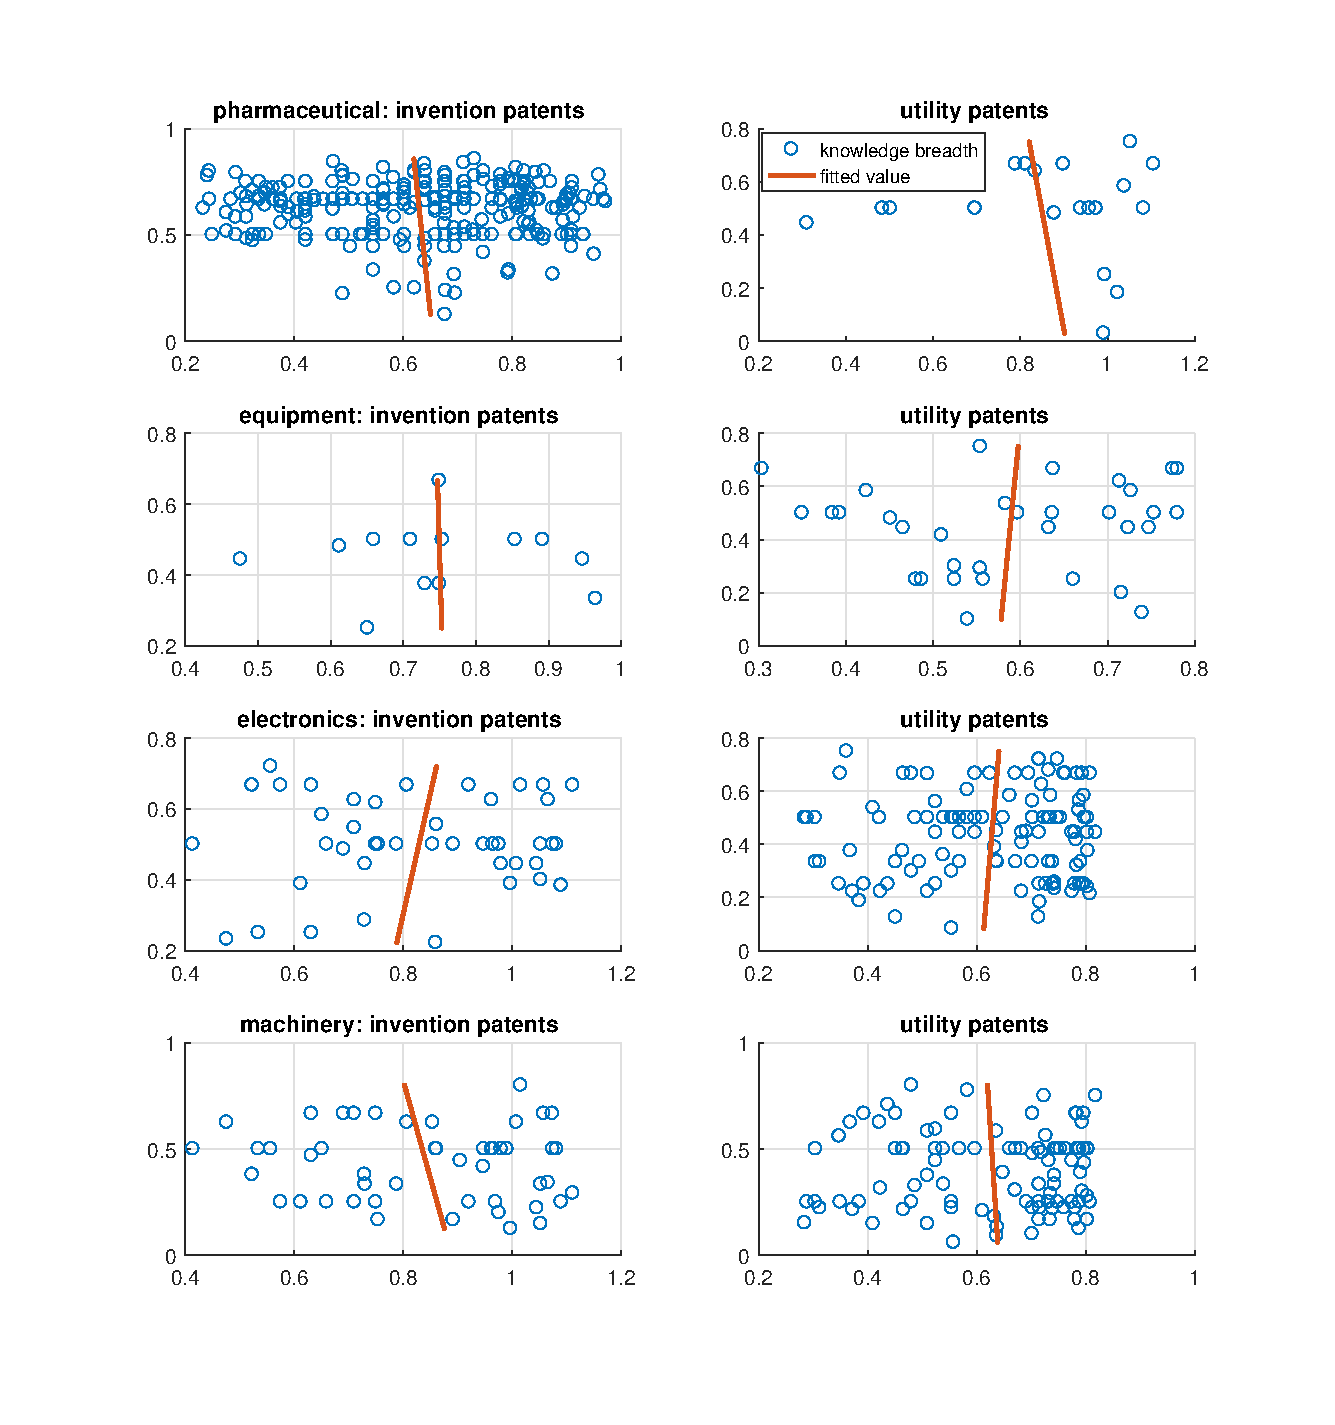
\includegraphics[width=0.6\textwidth]{Figs/patcorr.eps}
    \par\end{centering}
    \caption*{\small{}Note: quality measure is based on \citet{Dang2015}. In all graphs, the horizontal axis is the patent quality measure based on the knowledge width of the patent claim, the vertical axis is the model-generated patent value.}{\small \par}
    \end{figure}

\bibliographystyle{chicago}
\bibliography{bibref.bib}

\end{document}